% -*- Mode:TeX -*-

%% IMPORTANT: The official thesis specifications are available at:
%%            http://libraries.mit.edu/archives/thesis-specs/

\documentclass[12pt,twoside]{mitthesis}
\pagestyle{plain}
\usepackage{booktabs}
\usepackage{cmap}
\usepackage{float}
\usepackage[T1]{fontenc}
\usepackage{graphicx}
\usepackage{hyperref}
\usepackage{lgrind}
\usepackage{minted}
\usepackage{pgfplots}
\pgfplotsset{compat=newest}
\usepackage{subcaption}
\usepackage{tabularx}
\usepackage{xcolor}
\usepackage[backend=bibtex,style=ieee,bibencoding=ascii,maxnames=6,minnames=3,maxcitenames=2,mincitenames=1]{biblatex}
\usepgfplotslibrary{statistics}

\addbibresource{main.bib}

\newcommand{\TODO}[1]{\textcolor{red}{TODO: #1}}
\newcommand{\code}[1]{\texttt{#1}}


% for tensorboard graphs, from https://github.com/tensorflow/tensorflow/issues/9024
\definecolor{color1}{RGB}{209, 27, 27}
\definecolor{color2}{RGB}{36, 123, 160}
\definecolor{color3}{RGB}{62, 147, 97}
\pgfplotscreateplotcyclelist{tb}{
    semithick,color1\\%
    semithick,color2\\%
    semithick,color3\\%
}
\pgfplotsset{
	cycle list name=tb,
	label style={font=\scriptsize},
	tick label style={font=\tiny},
 	legend style={font=\scriptsize},
	scaled x ticks=false,
	grid=both,
	grid style={solid,gray!30!white},
	axis x line* = bottom,
	axis y line* = left,
}

\begin{document}

% -*-latex-*-
% 
% For questions, comments, concerns or complaints:
% thesis@mit.edu
% 
%
% $Log: cover.tex,v $
% Revision 1.8  2008/05/13 15:02:15  jdreed
% Degree month is June, not May.  Added note about prevdegrees.
% Arthur Smith's title updated
%
% Revision 1.7  2001/02/08 18:53:16  boojum
% changed some \newpages to \cleardoublepages
%
% Revision 1.6  1999/10/21 14:49:31  boojum
% changed comment referring to documentstyle
%
% Revision 1.5  1999/10/21 14:39:04  boojum
% *** empty log message ***
%
% Revision 1.4  1997/04/18  17:54:10  othomas
% added page numbers on abstract and cover, and made 1 abstract
% page the default rather than 2.  (anne hunter tells me this
% is the new institute standard.)
%
% Revision 1.4  1997/04/18  17:54:10  othomas
% added page numbers on abstract and cover, and made 1 abstract
% page the default rather than 2.  (anne hunter tells me this
% is the new institute standard.)
%
% Revision 1.3  93/05/17  17:06:29  starflt
% Added acknowledgements section (suggested by tompalka)
% 
% Revision 1.2  92/04/22  13:13:13  epeisach
% Fixes for 1991 course 6 requirements
% Phrase "and to grant others the right to do so" has been added to 
% permission clause
% Second copy of abstract is not counted as separate pages so numbering works
% out
% 
% Revision 1.1  92/04/22  13:08:20  epeisach

% NOTE:
% These templates make an effort to conform to the MIT Thesis specifications,
% however the specifications can change.  We recommend that you verify the
% layout of your title page with your thesis advisor and/or the MIT 
% Libraries before printing your final copy.
\title{\TODO{} thesis title hi hi hi}

\author{Kimberli Zhong}
% If you wish to list your previous degrees on the cover page, use the 
% previous degrees command:
%       \prevdegrees{A.A., Harvard University (1985)}
% You can use the \\ command to list multiple previous degrees
%       \prevdegrees{B.S., University of California (1978) \\
%                    S.M., Massachusetts Institute of Technology (1981)}
\department{Department of Electrical Engineering and Computer Science}

% If the thesis is for two degrees simultaneously, list them both
% separated by \and like this:
% \degree{Doctor of Philosophy \and Master of Science}
\degree{Bachelor of Science in Computer Science and Engineering}

% As of the 2007-08 academic year, valid degree months are September, 
% February, or June.  The default is June.
\degreemonth{June}
\degreeyear{2018}
\thesisdate{May 25, 2018}

%% By default, the thesis will be copyrighted to MIT.  If you need to copyright
%% the thesis to yourself, just specify the `vi' documentclass option.  If for
%% some reason you want to exactly specify the copyright notice text, you can
%% use the \copyrightnoticetext command.  
%\copyrightnoticetext{\copyright IBM, 1990.  Do not open till Xmas.}

% If there is more than one supervisor, use the \supervisor command
% once for each.
\supervisor{William J. Dally}{Associate Professor}

% This is the department committee chairman, not the thesis committee
% chairman.  You should replace this with your Department's Committee
% Chairman.
\chairman{Arthur C. Smith}{Chairman, Department Committee on Graduate Theses}

% Make the titlepage based on the above information.  If you need
% something special and can't use the standard form, you can specify
% the exact text of the titlepage yourself.  Put it in a titlepage
% environment and leave blank lines where you want vertical space.
% The spaces will be adjusted to fill the entire page.  The dotted
% lines for the signatures are made with the \signature command.
\maketitle

% The abstractpage environment sets up everything on the page except
% the text itself.  The title and other header material are put at the
% top of the page, and the supervisors are listed at the bottom.  A
% new page is begun both before and after.  Of course, an abstract may
% be more than one page itself.  If you need more control over the
% format of the page, you can use the abstract environment, which puts
% the word "Abstract" at the beginning and single spaces its text.

%% You can either \input (*not* \include) your abstract file, or you can put
%% the text of the abstract directly between the \begin{abstractpage} and
%% \end{abstractpage} commands.

% First copy: start a new page, and save the page number.
\cleardoublepage{}
% Uncomment the next line if you do NOT want a page number on your
% abstract and acknowledgments pages.
% \pagestyle{empty}
\setcounter{savepage}{\thepage}
\begin{abstractpage}
Today, designers work in tandem with computerized tools to create stylized graphic designs, diagrams, and icons.
In this work, we explore the applications of generative modeling to the design of vectorized drawings, with a focus on font glyphs.
We establish a data-driven approach for creating preliminary graphics upon which designers can iterate.
To accomplish this, we present an end-to-end pipeline for a supervised training system on Scalable Vector Graphics (SVGs) that learns to reconstruct training data and produce similar but novel examples.
We demonstrate its results on selected characters using a Google Fonts dataset of 2552 font faces.
Our approach uses a variational autoencoder to learn sequences of SVG drawing commands and is capable of both recreating ground truth inputs and generating unseen, editable SVG outputs.
To investigate improvements to model performance, we perform two experiments: one on the effects of various SVG feature encodings on generated outputs, and one on a modified architecture that explicitly encodes style and class separately for multi-class generation.

\end{abstractpage}

% Additional copy: start a new page, and reset the page number.  This way,
% the second copy of the abstract is not counted as separate pages.
% Uncomment the next 6 lines if you need two copies of the abstract
% page.
% \setcounter{page}{\thesavepage}
% \begin{abstractpage}
% Today, designers work in tandem with computerized tools to create stylized graphic designs, diagrams, and icons.
In this work, we explore the applications of generative modeling to the design of vectorized drawings, with a focus on font glyphs.
We establish a data-driven approach for creating preliminary graphics upon which designers can iterate.
To accomplish this, we present an end-to-end pipeline for a supervised training system on Scalable Vector Graphics (SVGs) that learns to reconstruct training data and produce similar but novel examples.
We demonstrate its results on selected characters using a Google Fonts dataset of 2552 font faces.
Our approach uses a variational autoencoder to learn sequences of SVG drawing commands and is capable of both recreating ground truth inputs and generating unseen, editable SVG outputs.
To investigate improvements to model performance, we perform two experiments: one on the effects of various SVG feature encodings on generated outputs, and one on a modified architecture that explicitly encodes style and class separately for multi-class generation.

% \end{abstractpage}

\cleardoublepage{}

\section*{Acknowledgments}

This is the acknowledgements section.  You should replace this with your
own acknowledgements.

%%%%%%%%%%%%%%%%%%%%%%%%%%%%%%%%%%%%%%%%%%%%%%%%%%%%%%%%%%%%%%%%%%%%%%
% -*-latex-*-

\pagestyle{plain}
  % -*- Mode:TeX -*-
%% This file simply contains the commands that actually generate the table of
%% contents and lists of figures and tables.  You can omit any or all of
%% these files by simply taking out the appropriate command.  For more
%% information on these files, see appendix C.3.3 of the LaTeX manual. 
\tableofcontents
\newpage
\listoffigures
\newpage
\listoftables


\TODO{run spell check}
\chapter{Introduction}

\TODO{hook}

Our motivation for examining the \textit{generation} of designs is two-fold.
One, we see practical purpose in a recommendation tool that augments a designer's experience, and we believe such a tool would be a valuable addition to a designer's creative process.
Two, we believe demystifying their generation would further solidify understanding of the intent and structure of human-created designs.
In algorithmically mimicking the process by which glyphs are created, we hope to gain a deeper grasp of from where humans' notion of design and style arises.

Although many strides have been made in understanding and synthesizing rasterized images and designs, primarily with convolutional neural networks, we focus our investigation on the domain of vectorized images in this work.
The two representations are quite different, and we aim to both produce generated designs with fewer aesthetically displeasing artifacts as well as investigate what new information about designs' underlying shapes and structures can be quantified and learned with the vectorized data format.

In the next chapter, we provide further background on the domain and discuss related work.
Then, in the following chapters, we delve into the methods used to train our vector graphics generator on the data processing side as well as the model architecture side.
We then demonstrate our methods as applied to font glyph generation, using a single-class as well as a multi-class approach.
Finally, we evaluate our results quantitatively and qualitatively and consider future directions of work.

\chapter{Background}
The problem space we explore ties together work across a number of different disciplines, including graphics, graphic design, and machine learning modeling.
In applying generative methods to vectorized glyphs, we are inspired by previous work in computer vision on non-natural images and draw upon recent developments in the generative modeling of line drawings.

\section{Non-natural images}
While natural images are photographs of real-world scenes and objects, non-natural images are computationally generated, either by hand with a computer design tool or automatically.
Images in this category include graphs, pictograms, virtual scenes, graphic designs, and more.
Algorithmically understanding, summarizing, and synthesizing these images pose unique challenges because of the images' clean and deliberately drawn designs, amalgamation of distinct visual and textual elements, and purposeful or narrative nature.

While much attention has been focused on research problems like object recognition, scene segmentation, and classification on natural images, interest in applying computer vision methods to non-natural images has been growing.
Much progress has been made towards computationally understanding non-natural images on datasets including XML-encoded abstract scenes~\cite{wu2017neural}, comic strips~\cite{iyyer2016amazing}, and textbook diagrams~\cite{seo2014diagram}.
Recent work by our group has explored the space of infographics, complex diagrams composed of visual and textual elements that deliver a message~\cite{bylinskii2017understanding}.

\subsection{Font faces}
Within the space of non-natural images, we focus specifically on designer-crafted font faces.
Fonts are used to typeset text with particular styles and weights, and many types of fonts exist, including serif, sans serif, and handwriting style fonts (see Figure~\ref{fig:fonttypes}).
Each font is defined by a set of glyphs, which include letters, digits, symbols, and potentially other Unicode characters.
Within a font face, glyphs generally share the same style for properties like angles, curvature, presence of serifs, and stroke width.

\begin{figure}[h]
    \centering
	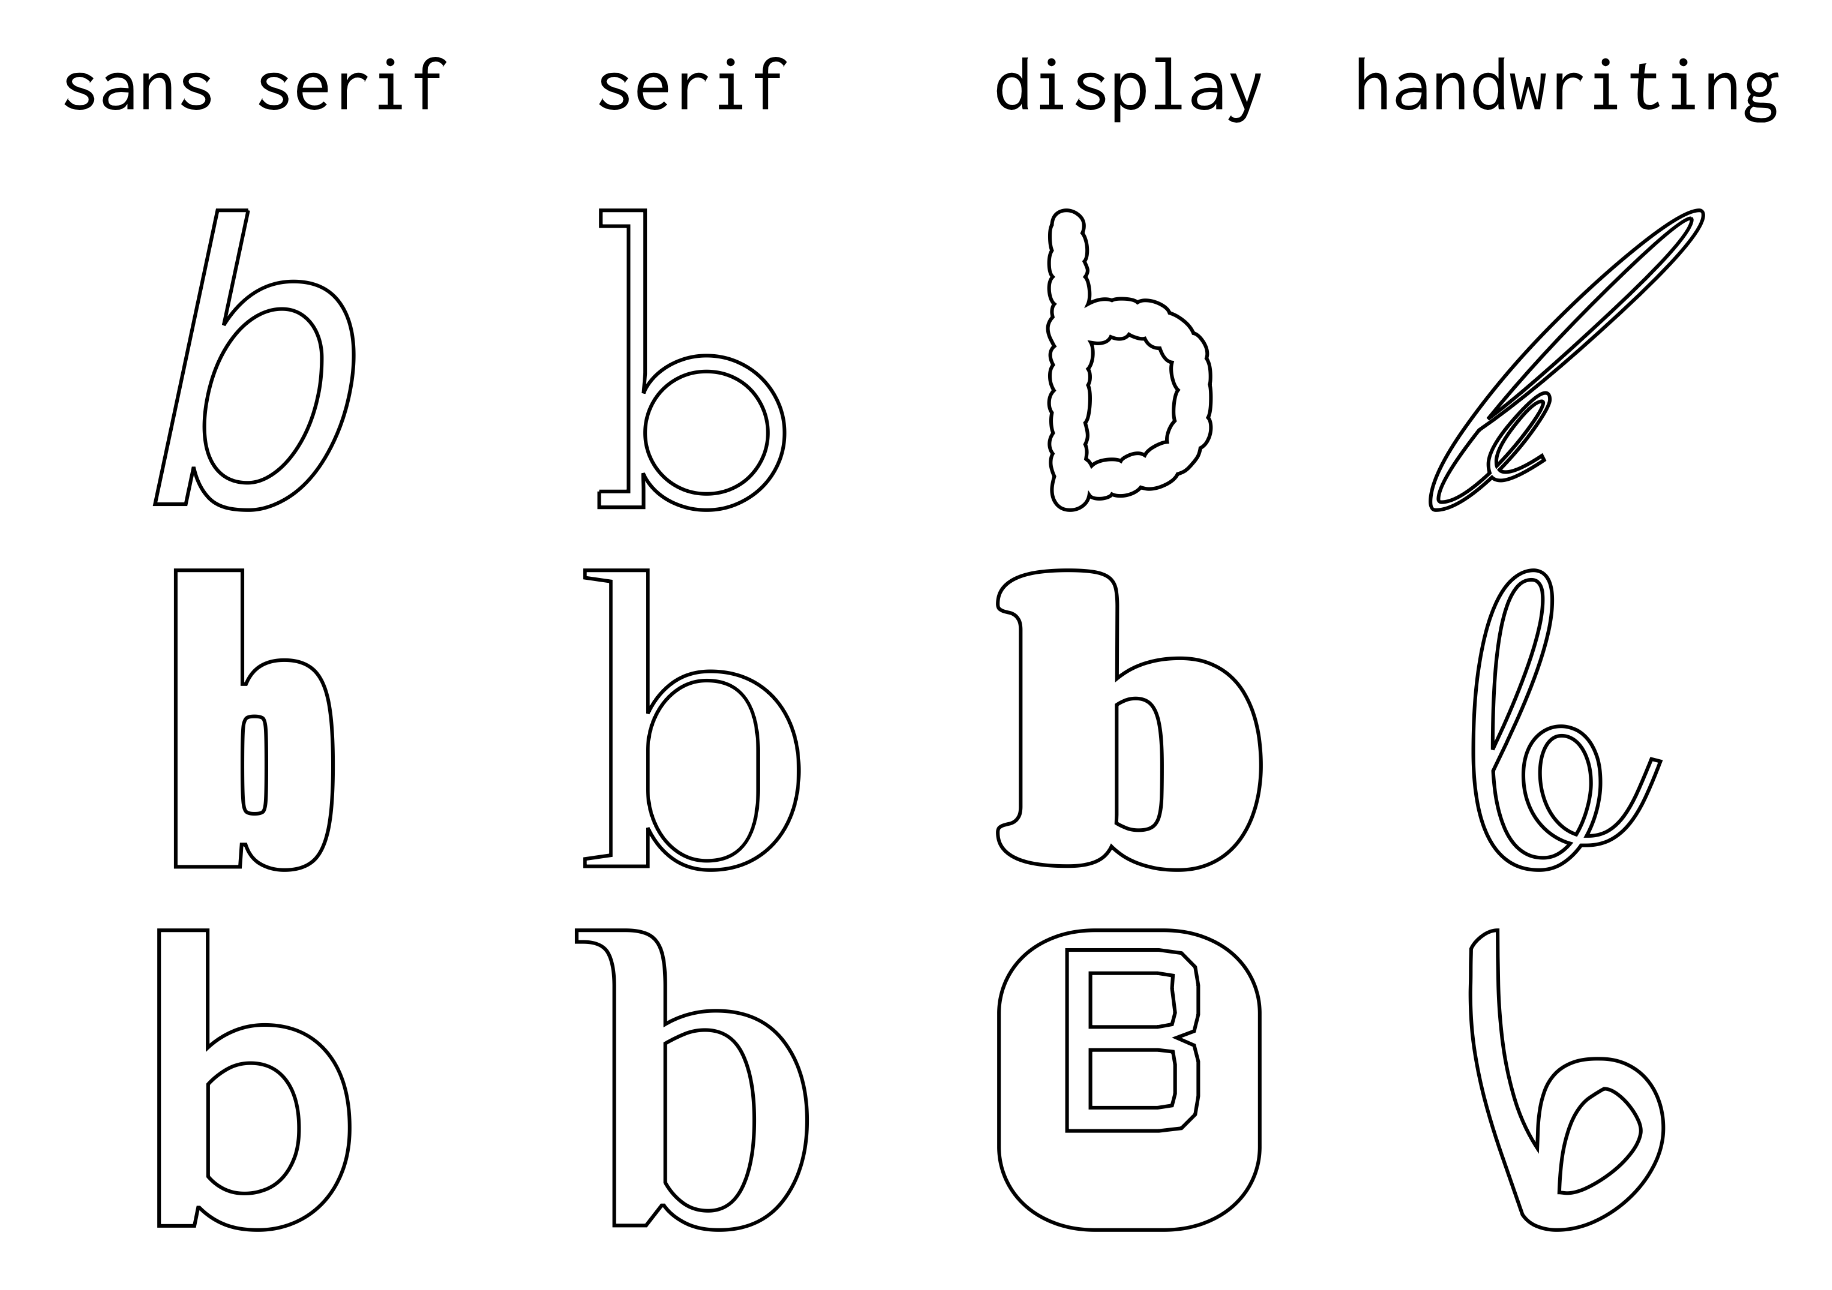
\includegraphics[width=0.55\textwidth]{figures/font_exs}
    \caption[Examples of glyphs from each font type]
    {Examples of glyphs from each font type. Serif glyphs have \textit{serifs}, or slight extensions off the ends of strokes, while sans serif glyphs do not.\label{fig:fonttypes}}
\end{figure}

In the context of computational modeling and generation, font glyphs offer certain advantages and pose distinctive challenges when compared to other types of designed graphics.
Unlike more complicated designs such as infographics and diagrams, they can be represented as drawings composed of simple lines and curves and, as such, can be modeled using sequential drawing commands.
However, font glyphs have distinct classes (i.e.\ each letter, number, symbol, etc.\ is a different class) and thus designing a generation procedure that is able to create clearly defined instances of different classes presents a challenge, as generation has to operate under strict constraints.

In this work, our computational methods are applied to font faces downloaded from Google Fonts\footnote{Downloaded from \url{https://github.com/google/fonts}, a GitHub repository containing all fonts in the dataset.}.
In Figure~\ref{fig:input_fonts}, a sampling of glyphs from the Google Fonts dataset is shown.

\begin{figure}[t]
	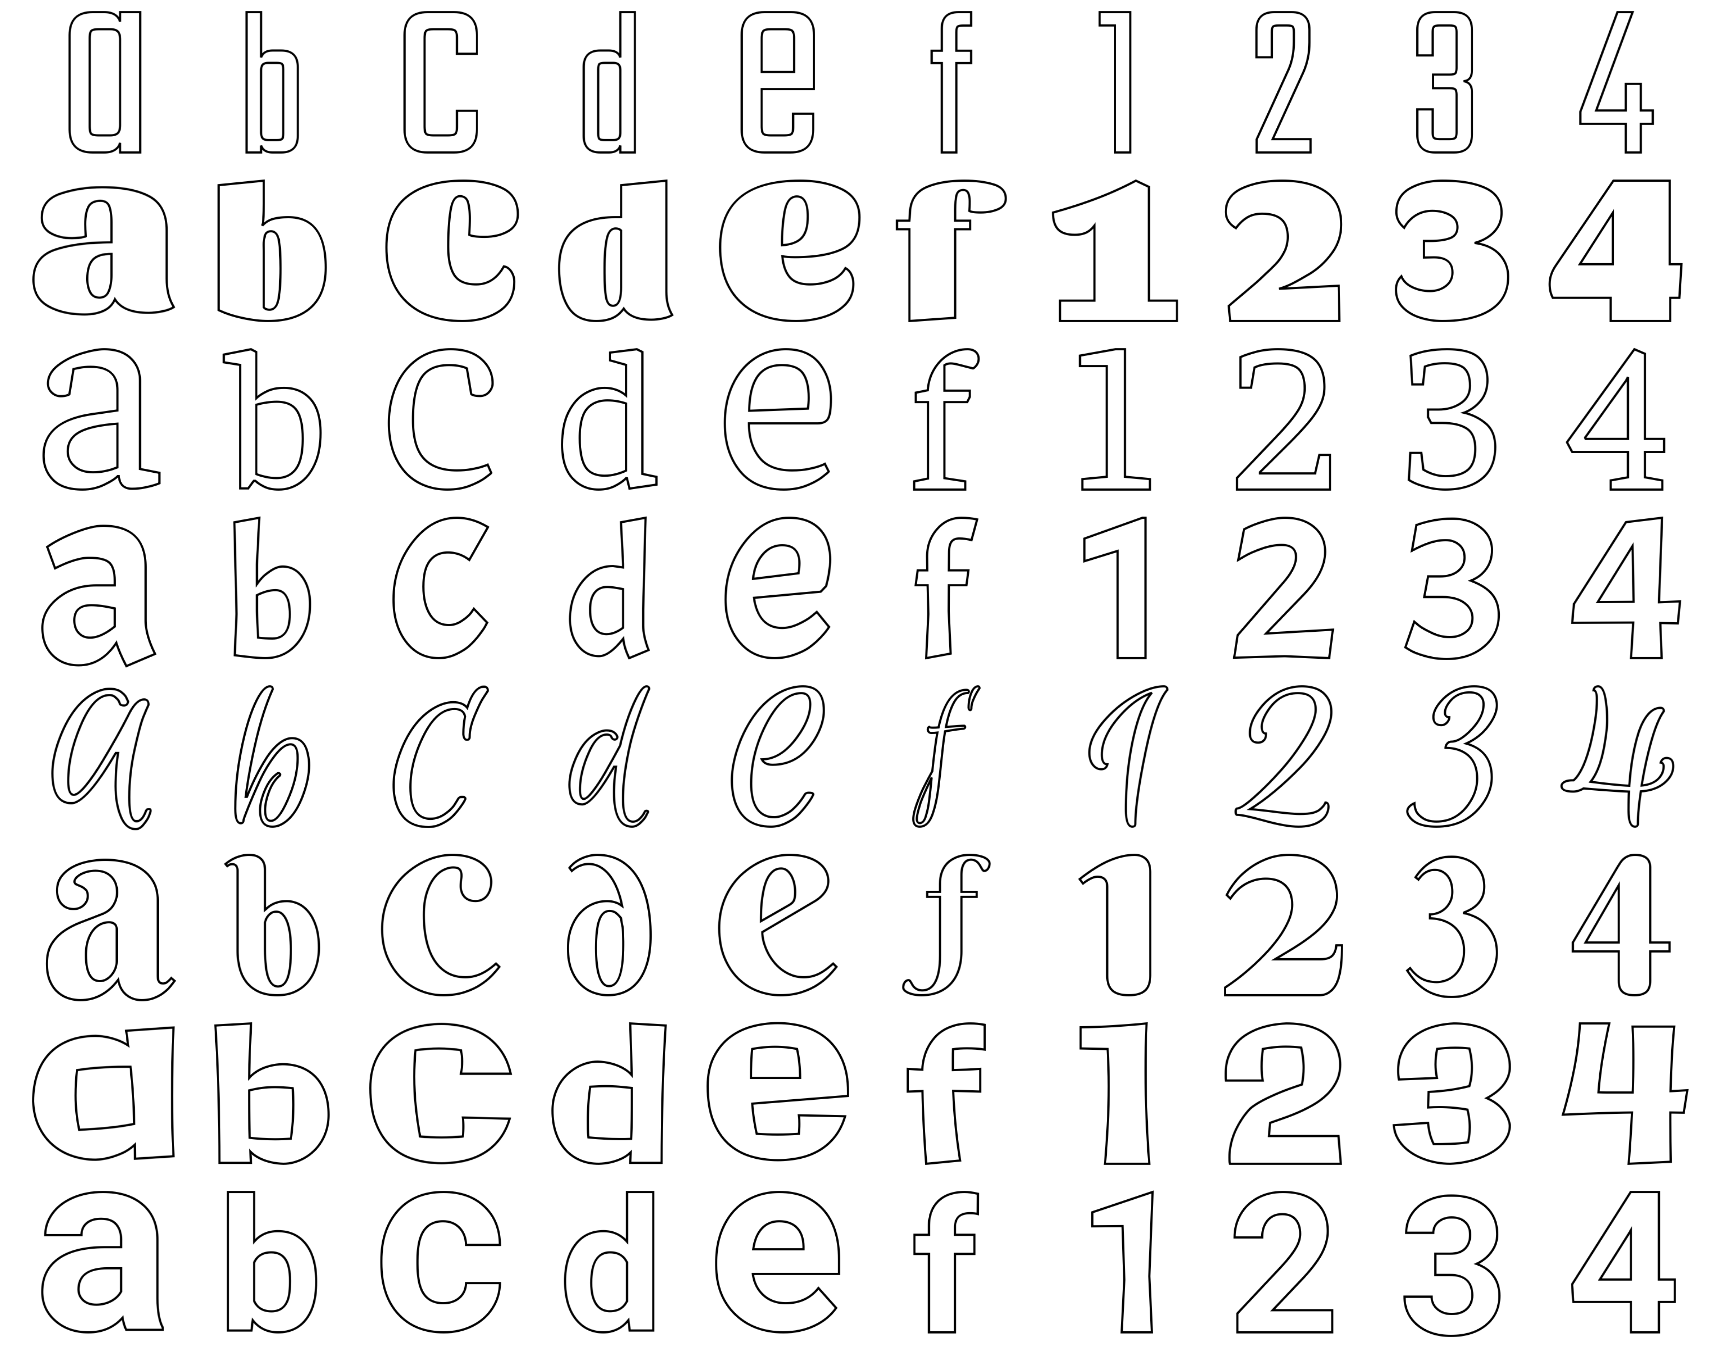
\includegraphics[width=\textwidth]{figures/input_fonts}
    \caption[A sample of the types of font faces used in our fonts dataset]{A sample of the types of font glyphs used in our dataset. Lowercase letters ``a'' through ``f'' are shown, as well as digits 1 through 4. Note the variety of styles represented: the dataset includes serif, sans serif, display, and handwriting style fonts.\label{fig:input_fonts}}
\end{figure}

\subsection{Vector graphics}
We are primarily interested in applying computational models to vector graphics as opposed to raster images.
While raster images encode color values for each point (or \textit{pixel}) in a two-dimensional grid, vector graphics describe a set of curves and shapes parameterized by mathematical equations and control points.
Many specifications exist for describing images in vector format, including SVG, Encapsulated PostScript (EPS), and Adobe PDF\@.
Font faces are often distributed as TrueType (TTF) files, which encode line and curve commands as well as metadata to aid with rendering.

Although the focus of our research is on font glyph inputs, our vision is to build a generalizable system for the variety of vector graphics generated by designers, including icons and logos.
Thus, our system accepts SVG data as input, as most vector graphics formats (including TTF) can be expressed using the commands available in the SVG specification.

\begin{figure}[t]
    \subcaptionbox{Raster images are defined as two-dimensional arrays of pixel values, while vector graphics define curves and paths mathematically. When scaled, vector graphics (right half) can still be rendered smoothly while raster images (left half) degrade in quality.\label{fig:svg-a}}
    {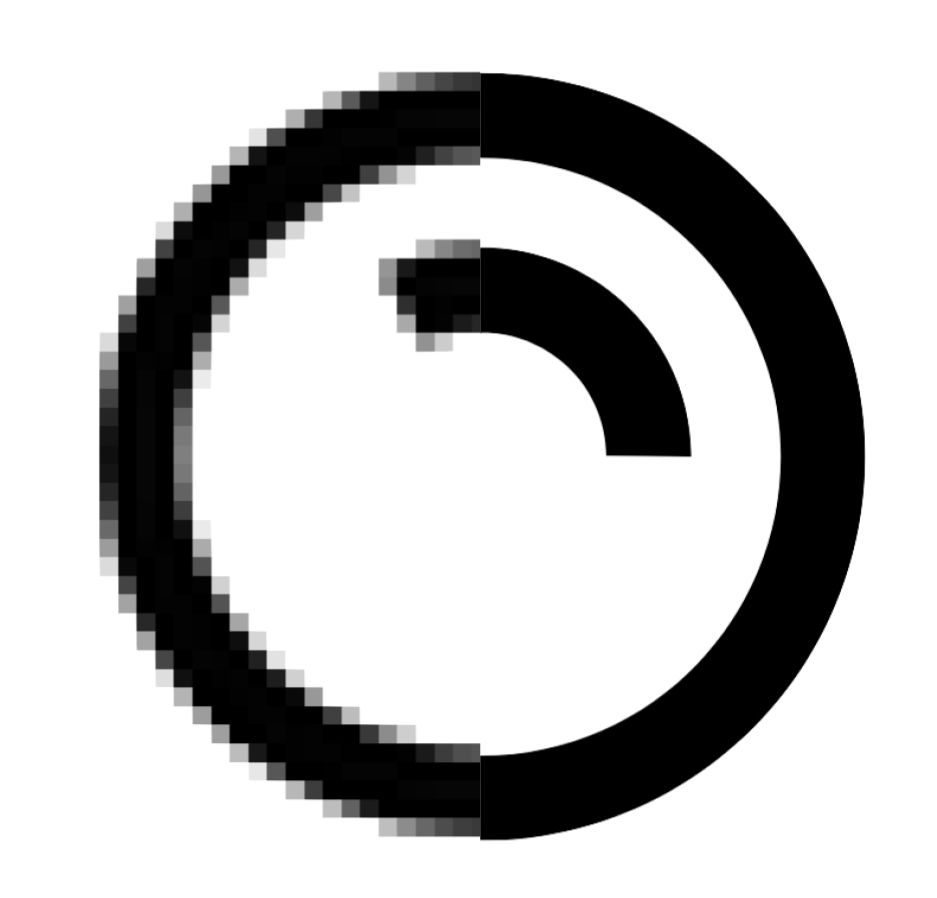
\includegraphics[height=1.85in]{figures/b_vs_vec}} \quad
    \subcaptionbox{SVG is an XML-based markup language that describes geometric elements within a vector image. A single path is used to draw this soap bubble, and colored curves in the image correspond approximately to the highlighted attribute commands that describe them. For example, the command \code{l-0.69-1.32} indicates a line drawn from a starting point to a point 0.69 units to the left and 1.32 units down.\label{fig:svg-b}}
    {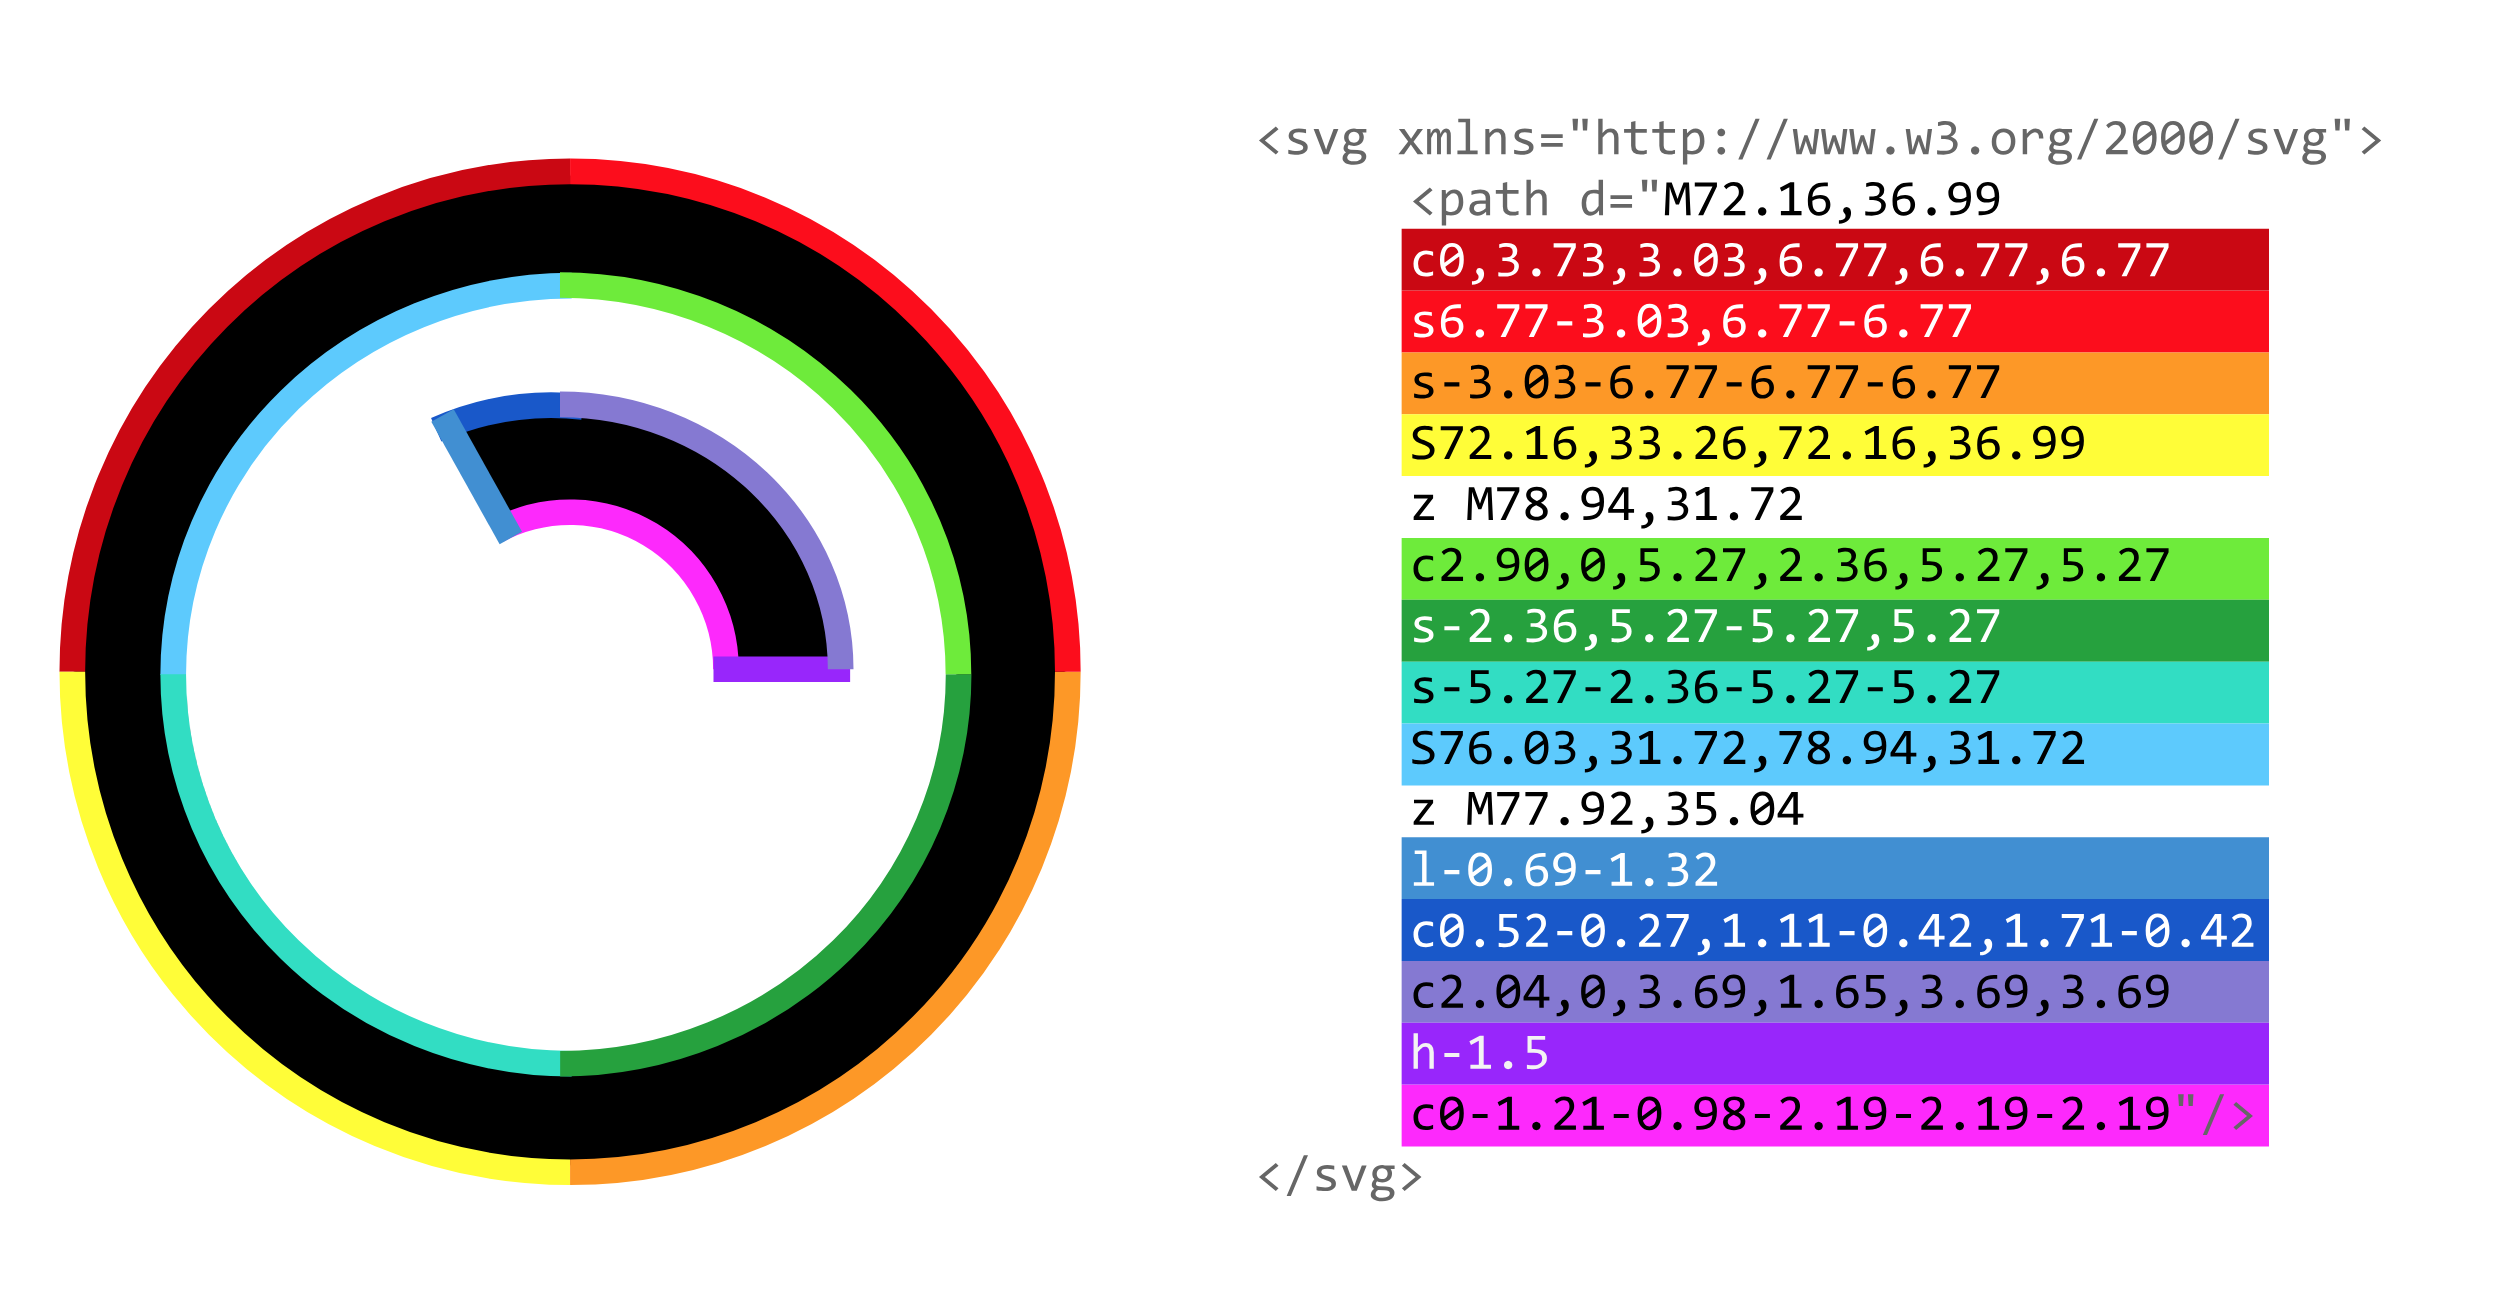
\includegraphics[height=1.85in]{figures/svgs}}
    \caption[An overview of vector graphics and Scalable Vector Graphics (SVG)]
    {A visual comparison of raster and vector graphics, and a sample SVG path.
    Image source: \textit{Dog Wash} by Llisole from the Noun Project.\label{fig:svg}}
\end{figure}

\subsubsection{Modeling vector graphics}
Applying computer vision techniques to vector graphics raises new challenges.
While bitmap and vector data can both decode into the same visual output, their underlying encoding structures have vast differences (Figure~\ref{fig:svg-a}).
As a data format, SVGs describe lists of geometric objects (among other elements such as text which are outside the scope of this work), including lines, circles, polygons, and splines.
The SVG \code{path} element, in particular, can be used to create all other element shapes.
Its attributes describe a series of commands that move from point to point, drawing curves or lines between them, as shown in Figure~\ref{fig:svg-b}.

The early popular deep convolutional network architectures designed to classify natural images, such as in~\cite{krizhevsky2012imagenet} and~\cite{simonyan2014very}, were designed to take in length $M\times N$ input vectors whose values directly represent corresponding pixel values in size $M\times N$ pixel input images.
While this model works well for raster images, this fixed-dimension format is incompatible with SVG element lists because their paths can describe any number of different point locations.
Instead, SVGs as sequential, variable-length, structured text are better suited to representation in models such as recurrent neural nets (RNNs).
RNNs are designed to model temporal sequences by unraveling across timesteps; long short-term memory (LSTM) models in particular use gated units to optimize for learning longer term dependencies~\cite{hochreiter1997long}.

\section{Generative modeling}
To solve the problem of creating novel vector drawings, we look towards the tools provided by generative machine learning methods.
While discriminative modeling techniques focus on separating and identifying inputs to produce output labels learned from high-dimensional data such as images, generative algorithms create previously unseen instances of a class based on representative inputs.
They are trained in an unsupervised or semi-supervised manner to learn a data distribution $P$, estimating the true data distribution $P_{gt}$ from which samples are drawn.
By drawing probabilistically from $P$, they can then be used to synthesize novel, unseen examples similar to input data.

Popular neural network-based approaches include generative-adversarial networks (GANs)~\cite{karpathy2016generative} and variational autoencoders (VAEs).
Introduced in~\citeyear{goodfellow2014generative}~\cite{goodfellow2014generative}, GANs pit a generative model $G(z; \theta_g)$ against an adversary $D(x; \theta_d)$ that learns to discriminate between samples from the ground truth dataset and the generative model's latent space.
When both $G$ and $D$ model differentiable functions, backpropagation can be used to train them towards convergence in a computationally efficient manner.

\subsection{Variational autoencoders}
Variational autoencoders, introduced in~\cite{kingma2013auto}, learn an encoder function mapping training examples from the input space $\mathcal{X}$ to vectors $z$ in the latent space $\mathcal{Z}$, as well as a decoder function that takes $z$ vectors sampled from a probability distribution $P(z)$ and applies a function that produces a random vector in the space $\mathcal{X}$~\cite{doersch2016tutorial}.
Intuitively, the goal is to train the model to produce outputs that look similar to the $x$ inputs but can be generated with some random noise such that they are distinct from training inputs.
To accomplish this goal, training a VAE tunes parameters $\theta$ to maximize the likelihood of reconstructing training examples after passing them through the entire pipeline, since increasing the probability of recreating $x$ inputs also increases the probability of creating similar random outputs.
Formally, we aim to maximize

\begin{equation}
    P(x) = \int P(x|\theta; z) P(z) dz
\end{equation}

Often, $P(x|\theta; z) = \mathcal{N}(x|f(\theta; z), \sigma^2 *I)$ where $\sigma$ is a parameter that can be set to manipulate the divergence of the generated output from training examples. In training, we constrain $P(z) = \mathcal{N}(0, 1)$ to simplify the loss calculation. 

Transforming this objective function to be differentiable and thus trainable using stochastic gradient descent requires a key insight: instead of sampling many $z_i$ then averaging $P(x|z_i)$, we focus only on the $z$ values that are likely to produce $x$ and compute $P(x)$ from those.
Our encoder then learns $Q(z|x; \phi)$ that approximates $P(z|x)$, while the decoder learns $P(x|z; \theta)$.
We can then define a loss function that describes a variational lower bound, where Kullback-Leibler (KL) divergence $\mathcal{D}$ accounts for the similarity between our $Q(z|x; \phi)$ and the true $P(z)$ and the reconstruction loss accounts for similarity between input and output:

\begin{equation}
    \mathcal{L}_i = -E_{z\sim Q(z|x_i; \phi)} [\log P(x_i|z; \theta)] + \mathcal{D}(Q(z|x_i; \phi)||P(z))
\end{equation}

In~\cite{graves2013generating}, the reconstruction loss function is expanded to account for sequential inputs and outputs, combining log loss for each item in the sequence.
This adjusted reconstruction loss can be used in a recurrent VAE architecture, where encoders and decoders digest sequential data.

\section{Related work}
Our end-to-end SVG generation model is inspired by prior work in line drawing generation, as both domains share an underlying temporal data structure.
Furthermore, our application to font generation is preceded by a history of computational approaches to font parameterization and style classification.

\subsection{Generating drawings}
Unconditionally generating parameterized curves extends the established problem of polyline generation.
Thus, we look towards contributions in handwriting and sketch generation, such as \citeauthor{graves2013generating}'s RNN-based handwriting prediction and synthesis work~\cite{graves2013generating}.
DRAW, a system introduced in~\cite{gregor2015draw}, uses a pair of recurrent networks in an VAE architecture to model attention in MNIST character generation.
Recent work by \citeauthor{ganin2017synthesizing} uses a reinforcement learning approach to train an agent to draw sketches~\cite{ganin2017synthesizing}.

Polyline results can easily be vectorized to produce splines, as in~\cite{janssen1997adaptive} or~\cite{birdal2014novel}.
However, our approach aims to model the entire SVG input to directly produce ready-to-edit spline output.
In our work, we build upon the variational autoencoder method presented by~\citeauthor{ha2017neural} in~\cite{ha2017neural}.
We use a similar bidirectional sequence-to-sequence VAE, with an overall loss calculation that includes drawing location losses, pen state losses, and KL loss.

\subsection{Font style}
\citeauthor{knuth1979tex}'s Metafont format demonstrates pioneering work in font style parameterization and has since motivated high-level font classification systems with font faces parameterized by human-controlled features like curvature and stroke width~\cite{knuth1979tex}\cite{lau2009learning}\cite{hassan2010next}.

Outside of manual feature selection approaches, many existing methods for modeling font style use font glyph raster images.
Tenenbaum and Freeman present a method for modeling style and content separately and apply it to font style extrapolation~\cite{tenenbaum1997separating}.
In~\cite{campbell2014learning}, polyline outlines are used to match glyphs across fonts using an energy optimization process, resulting in a learned manifold of fonts from which novel styles can be sampled.
Approaches for learning stylized calligraphy, such as~\cite{xu2005automatic}, take a more procedural approach, where strokes within characters are first extracted using shape segmentation approaches before use in training.
Neural network and VAE techniques to learning font style are increasingly common, such as in~\cite{upchurch2016z} and~\cite{wang2015deepfont}, and \citeauthor{lian2016automatic} use a combination of stroke segmentation and feature learning to generate handwriting fonts for Chinese characters~\cite{lian2016automatic}.

\chapter{SVG feature representation}\label{chap:features}
Our goal is to extend beyond polyline modeling and capture the higher-level shapes of SVG objects.
Thus, one major challenge is to choose an adequate representation that captures all drawing information from an SVG and can be fed as an input vector to our neural network architecture.
Although many different elements are allowed by the SVG specification, including text, images, and basic shapes, we simplify the problem space to focus only on the generic \code{path} element since paths can be used to compose other elements. 

\section{Overview of SVG commands}
There are five commands possible in an SVG \code{path} as seen in Figure~\ref{fig:svg-commands}. Further detail about command parameters can be found in Table~\ref{tbl:svg-commands}~\cite{grasso2011svg}.

\begin{figure}[h]
    \centering
	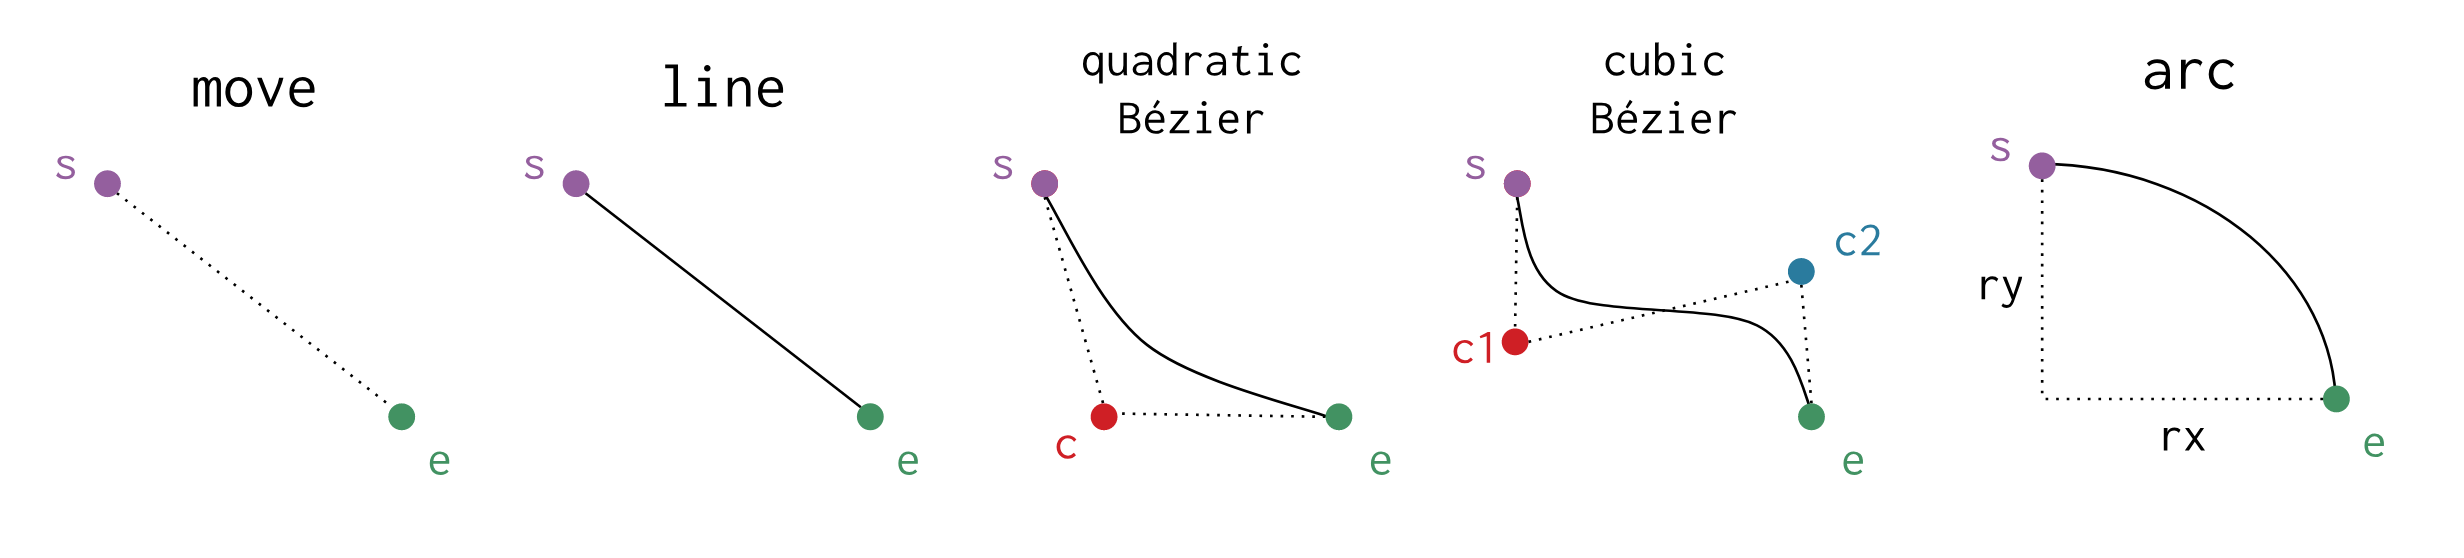
\includegraphics[width=\textwidth]{figures/commands}
    \caption{A visualization of the five commands in the SVG \code{path}\label{fig:svg-commands}}
\end{figure}


\begin{table}[h]
\centering
    \caption[The five possible commands in an SVG \code{path}]{A description of possible SVG path commands.
    For simplicity, we omit the relative coordinate variants of the commands, which specify $(dx, dy)$ coordinates instead of absolute $(x, y)$ for all control points.
    We also omit commands for vertical (\code{V}) and horizontal (\code{H}) lines as well as shorthand smoothed quadratic (\code{T}) and cubic (\code{S}) B\'eziers.\label{tbl:svg-commands}}
\begin{tabularx}{\linewidth}{l X}
\toprule
    Command & Code \& Description \\ \midrule
    Move & \code{M x y} \\
    & moves the pen to a specified point $(x, y)$ \\
    Line & \code{L x y} \\
    & draws a line from the current (start) point to the end point $(x, y)$ \\
    Quadratic B\'ezier & \code{Q cx cy, x y} \\
    & draws a quadratic B\'ezier curve according to given control point $(cx, cy)$ from the current point to the end point $(x, y)$ with the parametric equation $\textbf{B}(t) = (1-t)^2\textbf{s}+2(1-t)t\textbf{c} + t^2\textbf{e}$ \\
    Cubic B\'ezier & \code{C cx1 cy1, cx2 cy2, x y} \\
    & draws a cubic B\'ezier curve according to given control points $(cx_1, cy_1)$ and $(cx_2, cy_2)$ from the current point to the end point $(x, y)$ with the parametric equation $\textbf{B}(t) = (1-t)^3\textbf{s} + 3(1-t)^2t\textbf{c}_1 + 3(1-t)t^2\textbf{c}_2 + t^3\textbf{e}$\\
    Arc & \code{A rx ry t fl fs x y} \\
    & draws a section of an ellipse with the given $r_x$ and $r_y$ radii from the current point to the end point $(x, y)$ over angle $t$, with large-arc $f_l$ and sweep $f_s$ flags
\end{tabularx}
\end{table}

\section{Modeling SVGs}
We would like to model SVG inputs without loss of information about pen movements.
In essence, since SVGs name ordered lists of paths and their drawing commands, we model them as a sequence of mathematical parameters for the pen drawing commands and add a command for representing the transition between paths.
The sequential nature of this representation makes the generation task well-suited to a recurrent neural network architecture, as we cover in Chapter~\ref{chap:architecture}.

\subsection{Preprocessing}
SVG images often have additional properties like stroke and fill style.
As we focus on path generation exclusively, our first step in transforming input SVGs to a feature representation is to strip away those styles and focus only on the \code{path} elements of the input, often resulting in an image that depicts the outlines of the input shape---see Figure~\ref{fig:input_fonts} for examples.

Often, designers do not craft SVGs by editing XML by hand but rather with interactive image editing software such as Adobe Illustrator\footnote{\url{www.adobe.com/illustrator}} or Inkscape\footnote{\url{https://inkscape.org}}.
Thus, human-created SVGs often have varying path compositions, layers, and canvas sizes.

To constrain the modeling process, we first homogenize our dataset by preprocessing inputs, rescaling to the same overall canvas size (set to $256\times 256$ pixels) and reordering paths in the drawing sequence so that paths with larger bounding boxes are drawn first.

There is also variability in the directions and starting positions of path drawing.
Instead of controlling these factors in the preprocessing stage, our architecture is designed for bidirectionality, and all command sequences are interpreted such that the pen starts at coordinate $(0, 0)$ and moves to the first point in the input drawing.

\subsection{Simplifying path commands}
We aim to produce a system capable of modeling general SVGs, so inputs can contain any path command specified in Table~\ref{tbl:svg-commands}.
To avoid training bias and to constrain the problem space, we consolidate the different path commands into a single feature representation that encompasses all possible path pen movements.

Out of the five SVG path commands, three are parametic equations of differing degrees, so we can model these three (lines, quadratic B\'eziers, and cubic B\'eziers) using the parameter space for the highest degree cubic-order equation.
An elliptical arc segment, on the other hand, cannot be perfectly transformed into a cubic B\'ezier.
Arcs have five extra parameters used to describe them ($x$-radius, $y$-radius, angle of rotation, the large arc flag, and the sweep flag), so to compress their encoding we approximate them with the same parameter space as used for our parametric commands.
We use the method described in Appendix~\ref{app:algs} to approximate arc segments as cubic B\'eziers.

After all path drawing command types have been transformed to use the parameters needed for modeling cubic B\'ezier segments, we can represent each SVG command as a feature vector comprising those parameters and a three-dimensional one-hot pen state vector, similar to the feature representation used in~\cite{ha2017neural}.

Finally, for each \code{move} command and each disjoint path, we insert a feature vector that encodes the new end point and sets the pen state to note that the pen is up.

In all, our feature representation models each drawing command as a nine-dimensional vector (in contrast to the five-dimensional feature vector for polyline drawings in~\cite{ha2017neural}).
Six dimensions are used to model three $x, y$ coordinate parameters of cubic B\'eziers, and three dimensions are reserved for the pen up ($p_u$), pen down ($p_d$), and end drawing ($p_e$) pen states.
Each input SVG is transformed into a sequence of commands, which is in turn translated into a sequence of these feature vectors.
In Chapter~\ref{chap:feature-variation}, we examine further details of this feature transformation process and how our representation modifications affect modeling performance.

\chapter{Font glyph generation}
\section{Dataset collection}\label{sec:font-data}
\section{Model architecture}\label{sec:architecture}
\subsection{Single-class}
\subsection{Multi-class}
\section{Training}
\section{Results}
\begin{figure}[t]
	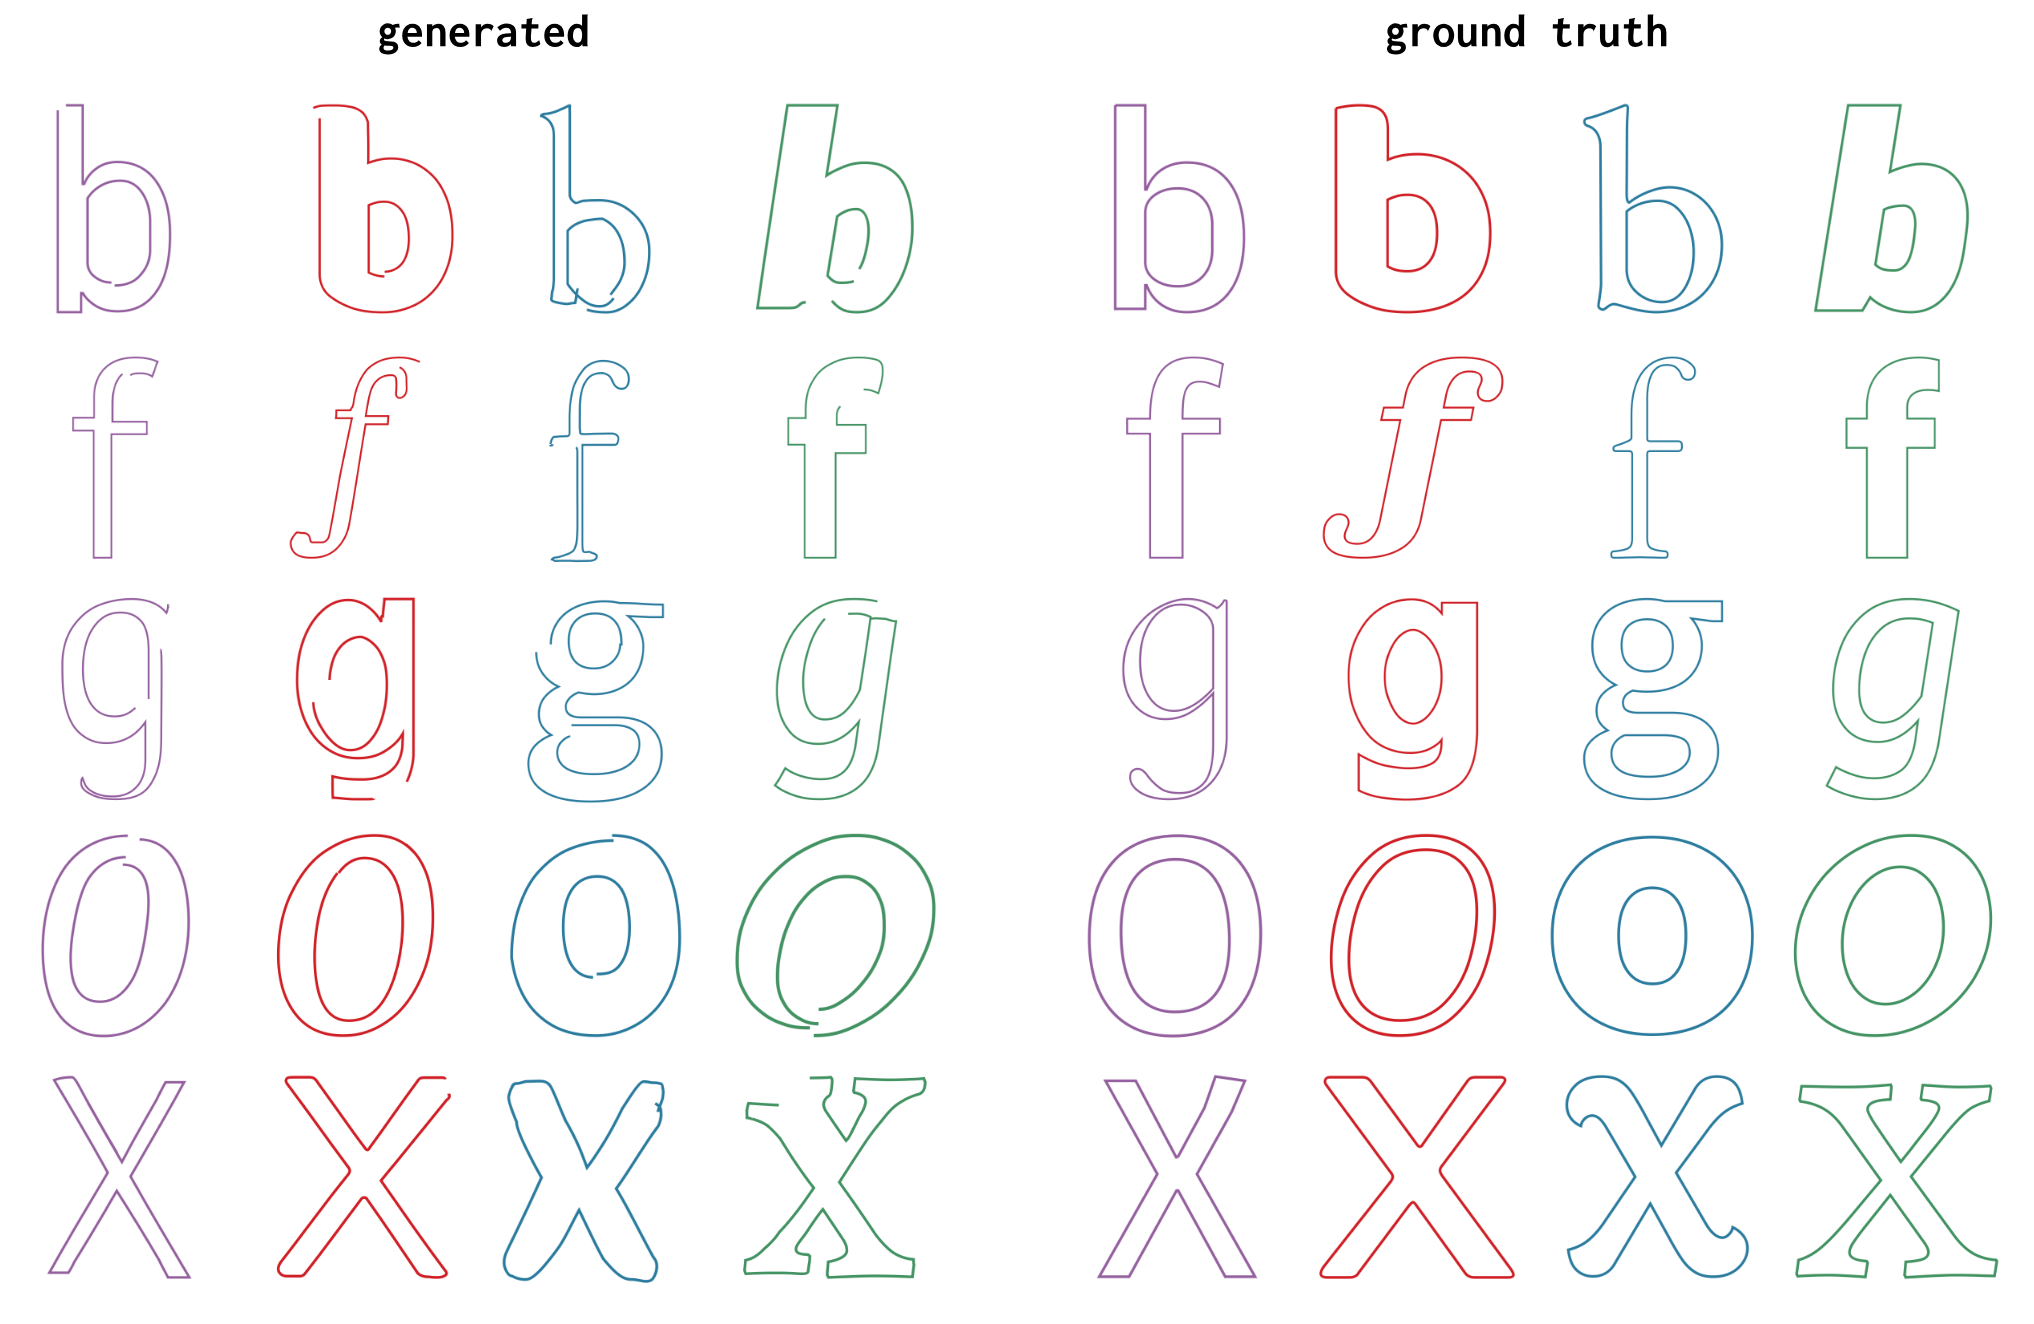
\includegraphics[width=\textwidth]{figures/font_gen}
    \caption[Visual results of training \TODO{blah}]{\TODO{caption}\label{fig:font_gen}}
\end{figure}

\chapter{Application: font glyph generation}\label{chap:training} To demonstrate our end-to-end SVG generation method, we train the model architecture described in Chapter~\ref{chap:architecture} on a dataset of font glyphs.

\section{Dataset}\label{sec:font-data}
Our dataset of font faces is downloaded from a GitHub repository containing all fonts available on Google Fonts (\url{https://github.com/google/fonts}).
The dataset contains 2552 font faces total from 877 font families.
Font faces exhibit much stylistic variation: a breakdown of font types for the 877 font families can be found in Table~\ref{tbl:fonttypes}, and examples of font glyphs from each type can be found in Figure~\ref{fig:fonttypes}.

\begin{table}[h]
\centering
\caption[A breakdown of font types in the Google Fonts dataset]
    {The 2552 font faces in the Google Fonts dataset are from 877 total font families.
    Each font family can be classified as one of the following categories, with the ``display'' category encompassing bold fonts of a wide variety of styles that can be used as title text.
    Here, we report the counts of font families in the dataset belonging to each type.\label{tbl:fonttypes}}
\begin{tabular}{c c c c c}
\toprule
    Serif & Sans serif & Display & Handwriting & Monospace \\ \midrule
    180 & 249 & 296 & 135 & 17
\end{tabular}
\end{table}

\begin{figure}[h]
    \centering
	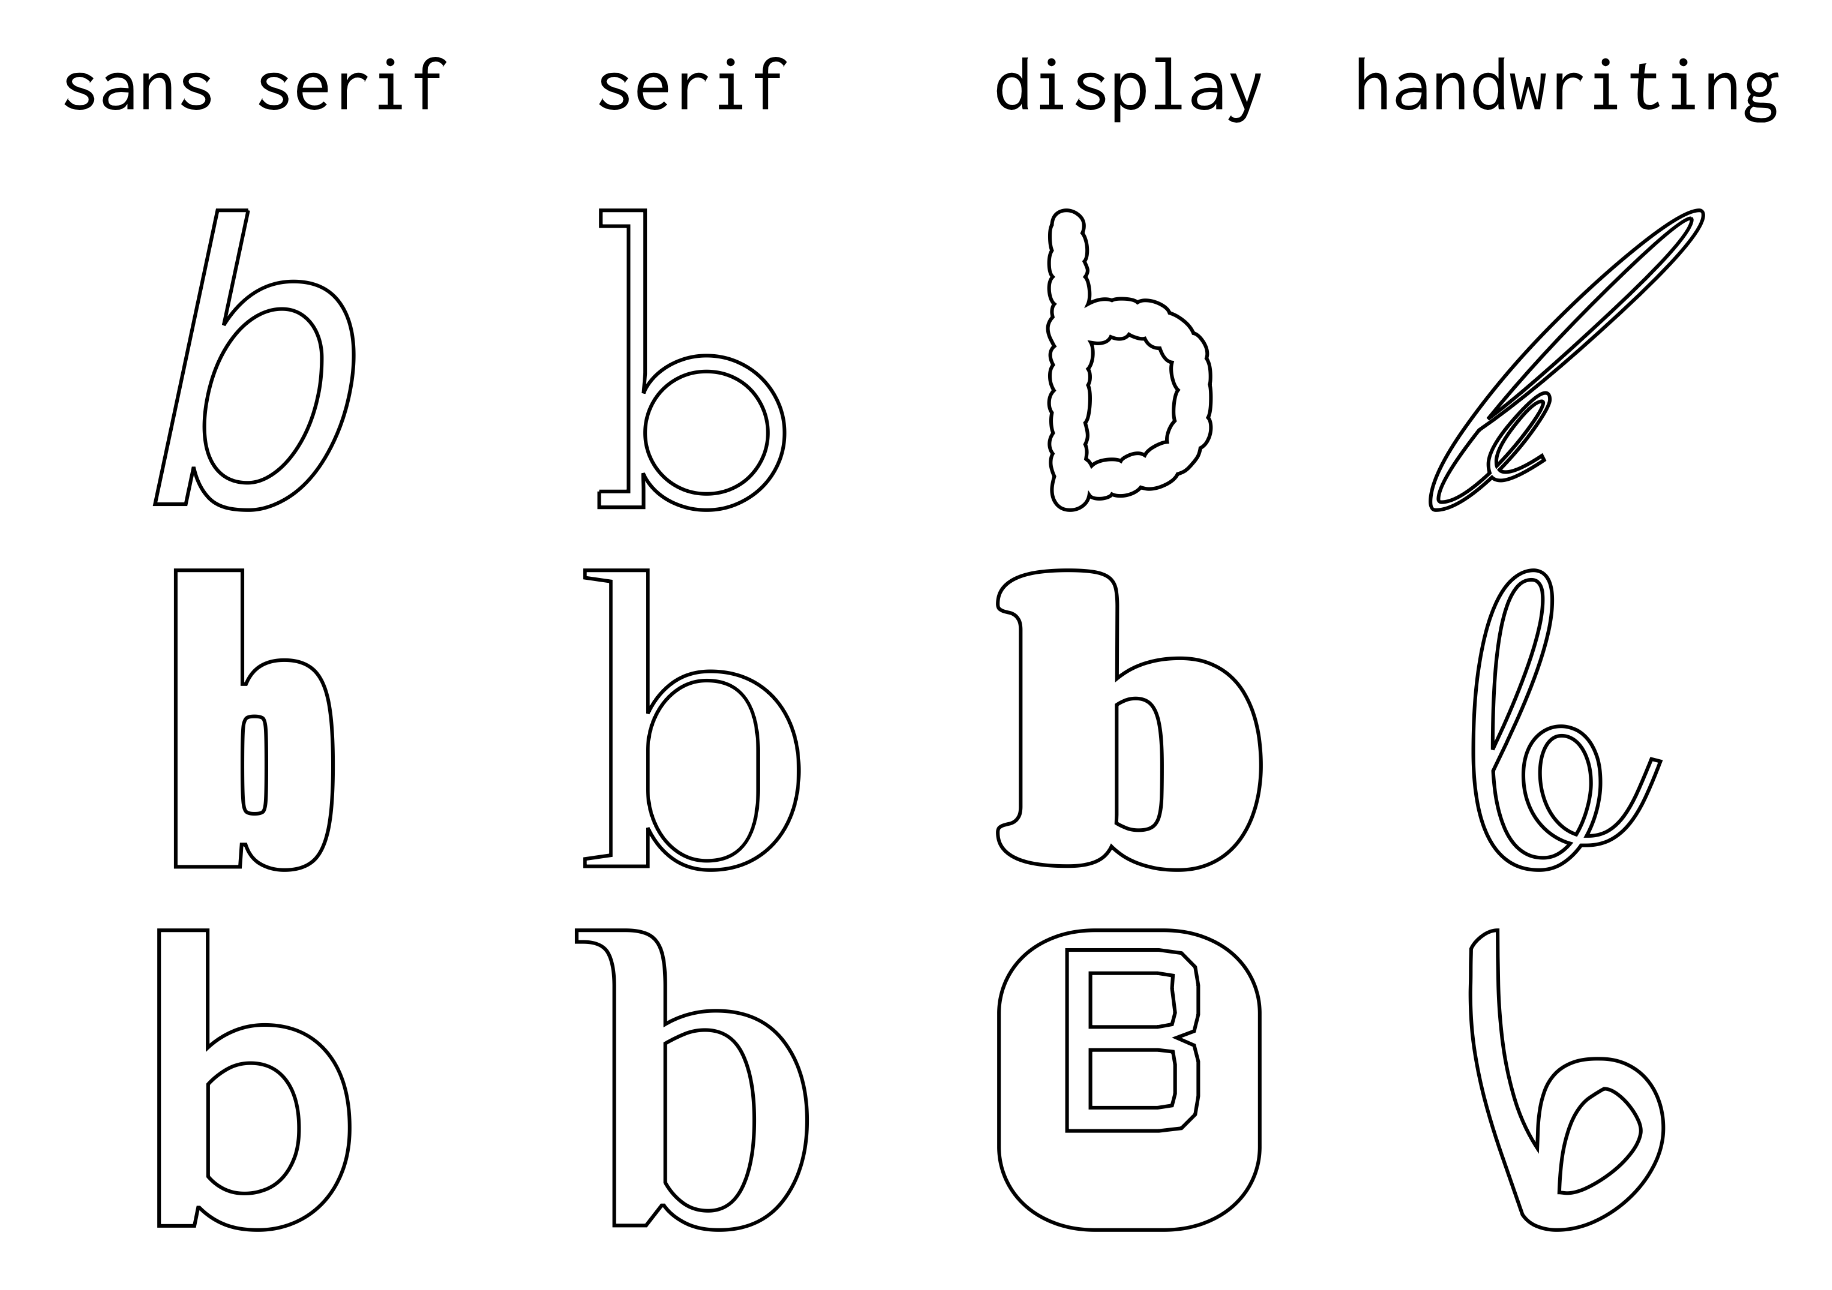
\includegraphics[width=\textwidth]{figures/font_exs}
    \caption[Examples of glyphs from each font type]
    {Examples of glyphs from each font type described in Table~\ref{tbl:fonttypes}.
    Note that we exclude examples from the ``monospace'' category, as the defining characteristic of that type is more about character spacing than style.\label{fig:fonttypes}}
\end{figure}

All font faces are downloaded as TTF files then converted to SVG format using the FontForge command-line tool\footnote{\url{https://fontforge.github.io}}.

The statistics for the glyph \textbf{b} across all font faces are shown in Figure~\ref{fig:stats-b}.
The remaining glyph statistics can be found in Appendix~\ref{app:data}.

\begin{figure}[h]
    \caption[Dataset statistics for the glyph \textbf{b}]
    {Dataset statistics for the glyph \textbf{b} across all 2552 font faces in the Google Fonts dataset.\label{fig:stats-b}}
\centering
\subcaptionbox*{}
{\begin{tikzpicture}
\begin{axis}[
 	xlabel={feature vector count},
    ylabel={number of \textbf{b} glyphs},
	width=0.45\textwidth,
    ybar,
    ymin=0
]
\addplot [
	fill=color1,
	fill opacity=0.4,
    hist={
        bins=7,
        data min=0.5,
        data max=300
    }   
] table [y index=0] {data/b_points_stats.csv};
\end{axis}
\end{tikzpicture}
}
\subcaptionbox*{}
{\begin{tikzpicture}
\begin{axis}[
 	xlabel={command type count},
    ylabel={number of \textbf{b} glyphs},
	width=0.45\textwidth,
    ybar,
    ymin=0
]
\addplot [
	fill=color2,
	fill opacity=0.4,
    hist={
        bins=7,
        data min=0.5,
        data max=100
    }   
] table [y index=0] {data/b_line_count.csv};
\addplot [
	fill=color3,
	fill opacity=0.4,
    hist={
        bins=7,
        data min=0.5,
        data max=100
    }   
] table [y index=0] {data/b_quad_count.csv};
\addlegendentry{\code{line}}
\addlegendentry{\code{quad}}
\end{axis}
\end{tikzpicture}
}
\end{figure}

\section{Training}
We train the model on single-class datasets for the glyphs \textbf{b}, \textbf{f}, \textbf{g}, \textbf{o}, and \textbf{x}, chosen because they cover a variety of shapes and curves.
Each input SVG is transformed to a list of feature vectors using the method described in Chapter~\ref{chap:features}.
We use encoding B, details of which are described in Chapter~\ref{chap:feature-variation}.
The datasets are then randomly partitioned into training, test, and validation sets; glyphs from the overall dataset of 2552 font faces are pruned if they consist of more than 250 feature vectors.
Every glyph except \textbf{x} has a training set of 1920 SVGs, while \textbf{x} has a training set of 1960.
All glyphs have test and validation sets of 240 SVGs each.
Training is done with a batch size of 40, a learning rate of 0.001, and a KL weight in the loss function that starts at 0.01 and increases slowly over time.
The size of the latent space vector $z$ is set to 128, and we use recurrent dropout to reduce overfitting.
Cost graphs and details about trained models can be found in Appendix~\ref{app:train}.

\section{Results}
Here, we report quantitative results as well as a qualitative evaluation of model performance.
\begin{figure}[h]
    \centering
	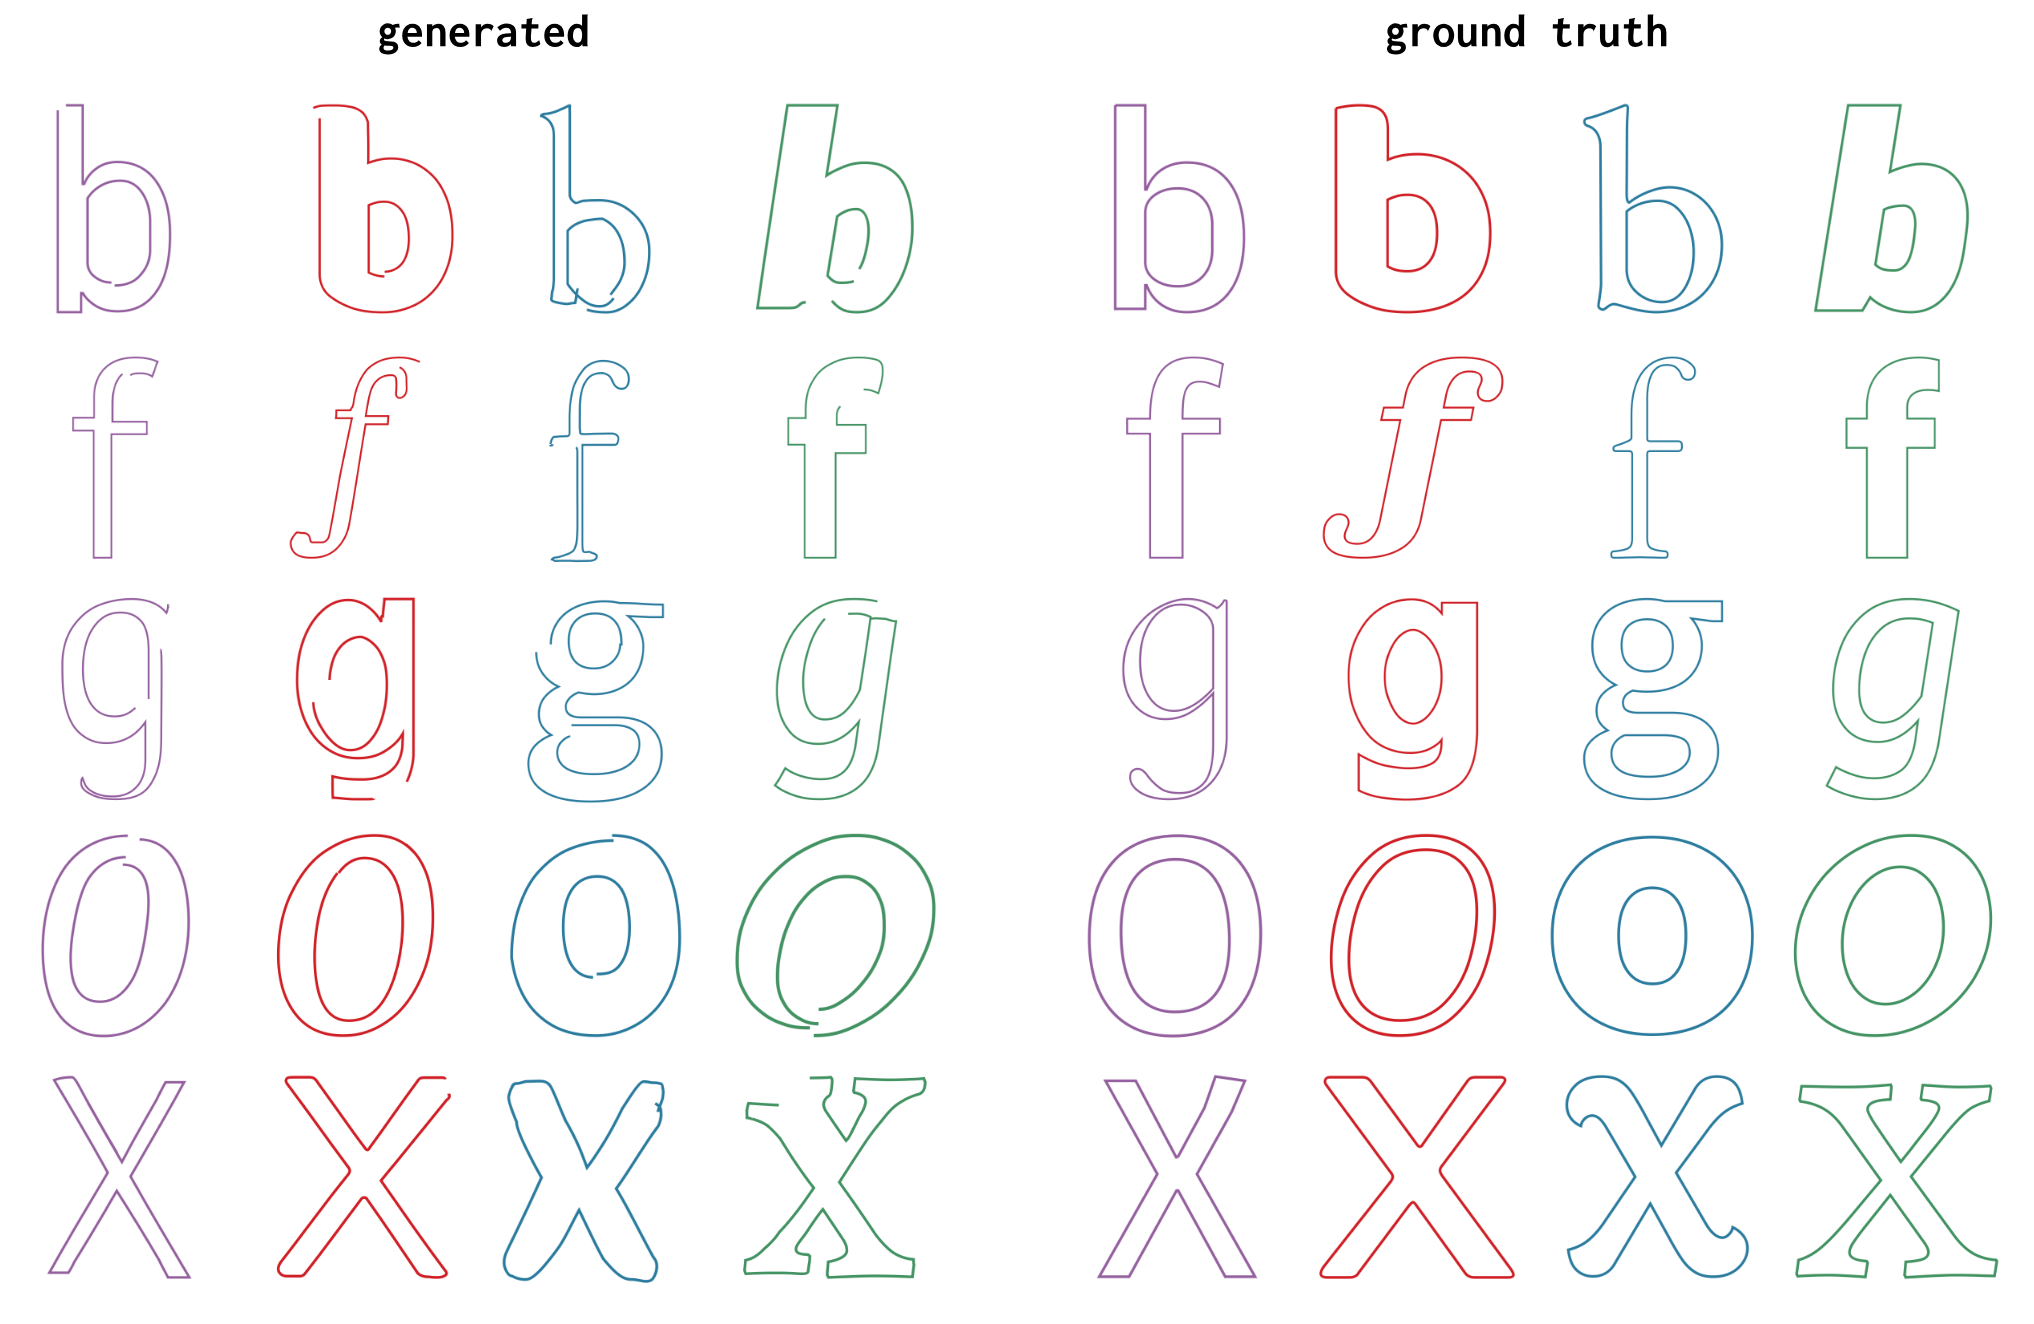
\includegraphics[width=\textwidth]{figures/font_gen}
    \caption[Visual results of training single-class model on letter glyph datasets]
    {Selected glyphs conditionally generated by the trained single-class model.
    Ground truth inputs on the right are fed into the encoder and decoded into the generated outputs on the left.\label{fig:font_gen}}
\end{figure}

\subsection{Quantitative results}\label{sec:quant-eval}
To quantify model performance, we compute an image similarity metric between each ground-truth image and a corresponding image conditionally generated by the model with $\tau = 0.3$, where temperature $\tau$ increases randomness when sampling from the decoder as defined in~\cite{ha2017neural}.
Images are first converted to point clouds containing every pixel in the raster image with nonzero value.
The resulting sets of points are translated to be mean-centered for each image, and the modified Hausdorff distance is calculated from the point set of each generated image to the point set of its corresponding ground truth image~\cite{dubuisson1994modified}.
While we also considered using metrics such as pixel loss and feature extraction, we chose the Hausdorff distance for its simplicity as a measure of mutual polygonal proximity.
Evaluation is run on a set of $N$ test images for each glyph, and quantitative results can be found in Table~\ref{tbl:model-results}.

\begin{table}[h]
\centering
\caption[Quantitative results for models trained on letter glyphs]
    {Modified Hausdorff distance for models trained on each glyph on a test set of $N$ images.\label{tbl:model-results}}
\begin{tabular}{c c c c c}
\toprule
    Glyph & Mean & Std.\ dev. & Kurtosis & $N$ \\ \midrule
    \textbf{b} & 19.5341 & 8.3484 & 1.9515 & 240 \\
    \textbf{f} & 15.7533 & 9.2132 & 4.7359 & 240 \\
    \textbf{g} & 19.7714 & 9.6469 & 6.8383 & 240 \\
    \textbf{o} & 27.8857 & 11.9887 & 5.8081 & 240 \\
    \textbf{x} & 28.8542 & 14.2474 & 1.9820 & 238 
\end{tabular}
\end{table}

\subsection{Qualitative results}
We demonstrate the model's learned ability with a few illustrative examples.

In Figure~\ref{fig:interp}, we interpolate between latent vectors for input \textbf{b} and \textbf{f} glyphs of different styles.
If interpolated latent vectors tend to produce coherent outputs, it indicates that the latent space is efficiently used and that the KL regularization term in the loss function has sufficient power.
\begin{figure}[h]
    \centering
	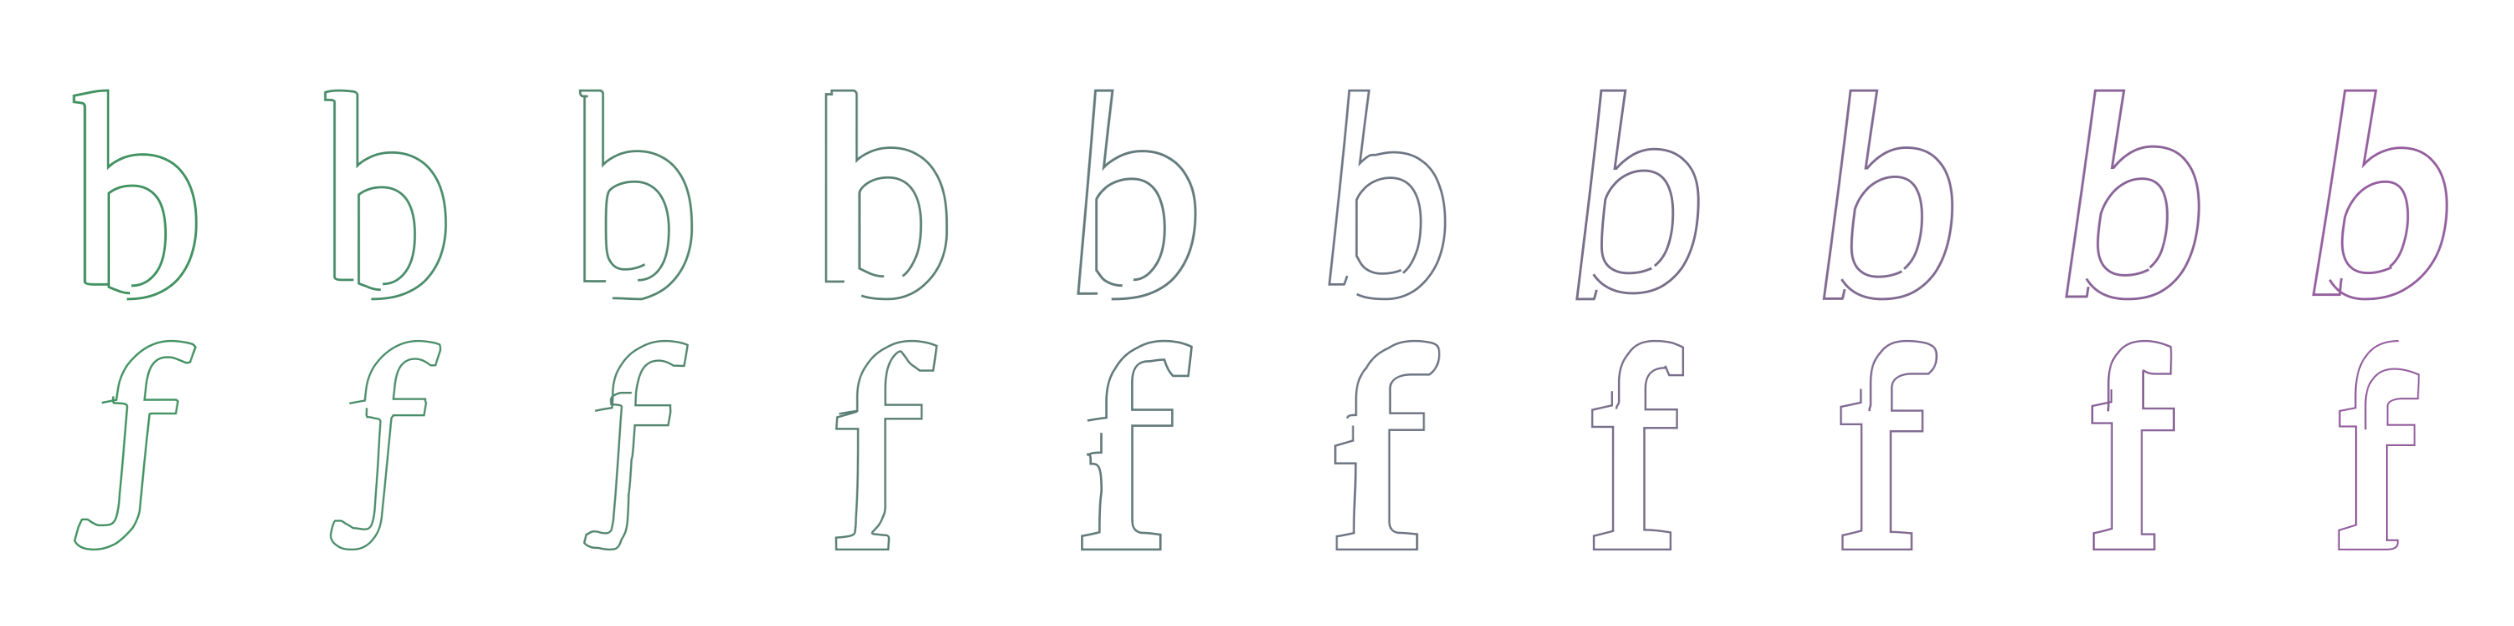
\includegraphics[width=\textwidth]{figures/interp}
    \caption[Latent space interpolation for the single-class model]
    {The latent space abstractly encodes both style and method---it must represent both how to draw a given glyph as well as the identify different types of glyphs.
    The input glyphs are on the far sides of the figure, and we spherically interpolate between their latent vectors, decoding with $\tau=0.1$.\label{fig:interp}}
\end{figure}

In Figure~\ref{fig:temp}, we demonstrate how temperature $\tau$ affects the decoding process as a scaling factor to $\sigma$ in the sampled GMMs. Intuitively, a lower temperature indicates that the decoder samples outputs that are believes are more likely.
\begin{figure}[h]
    \centering
	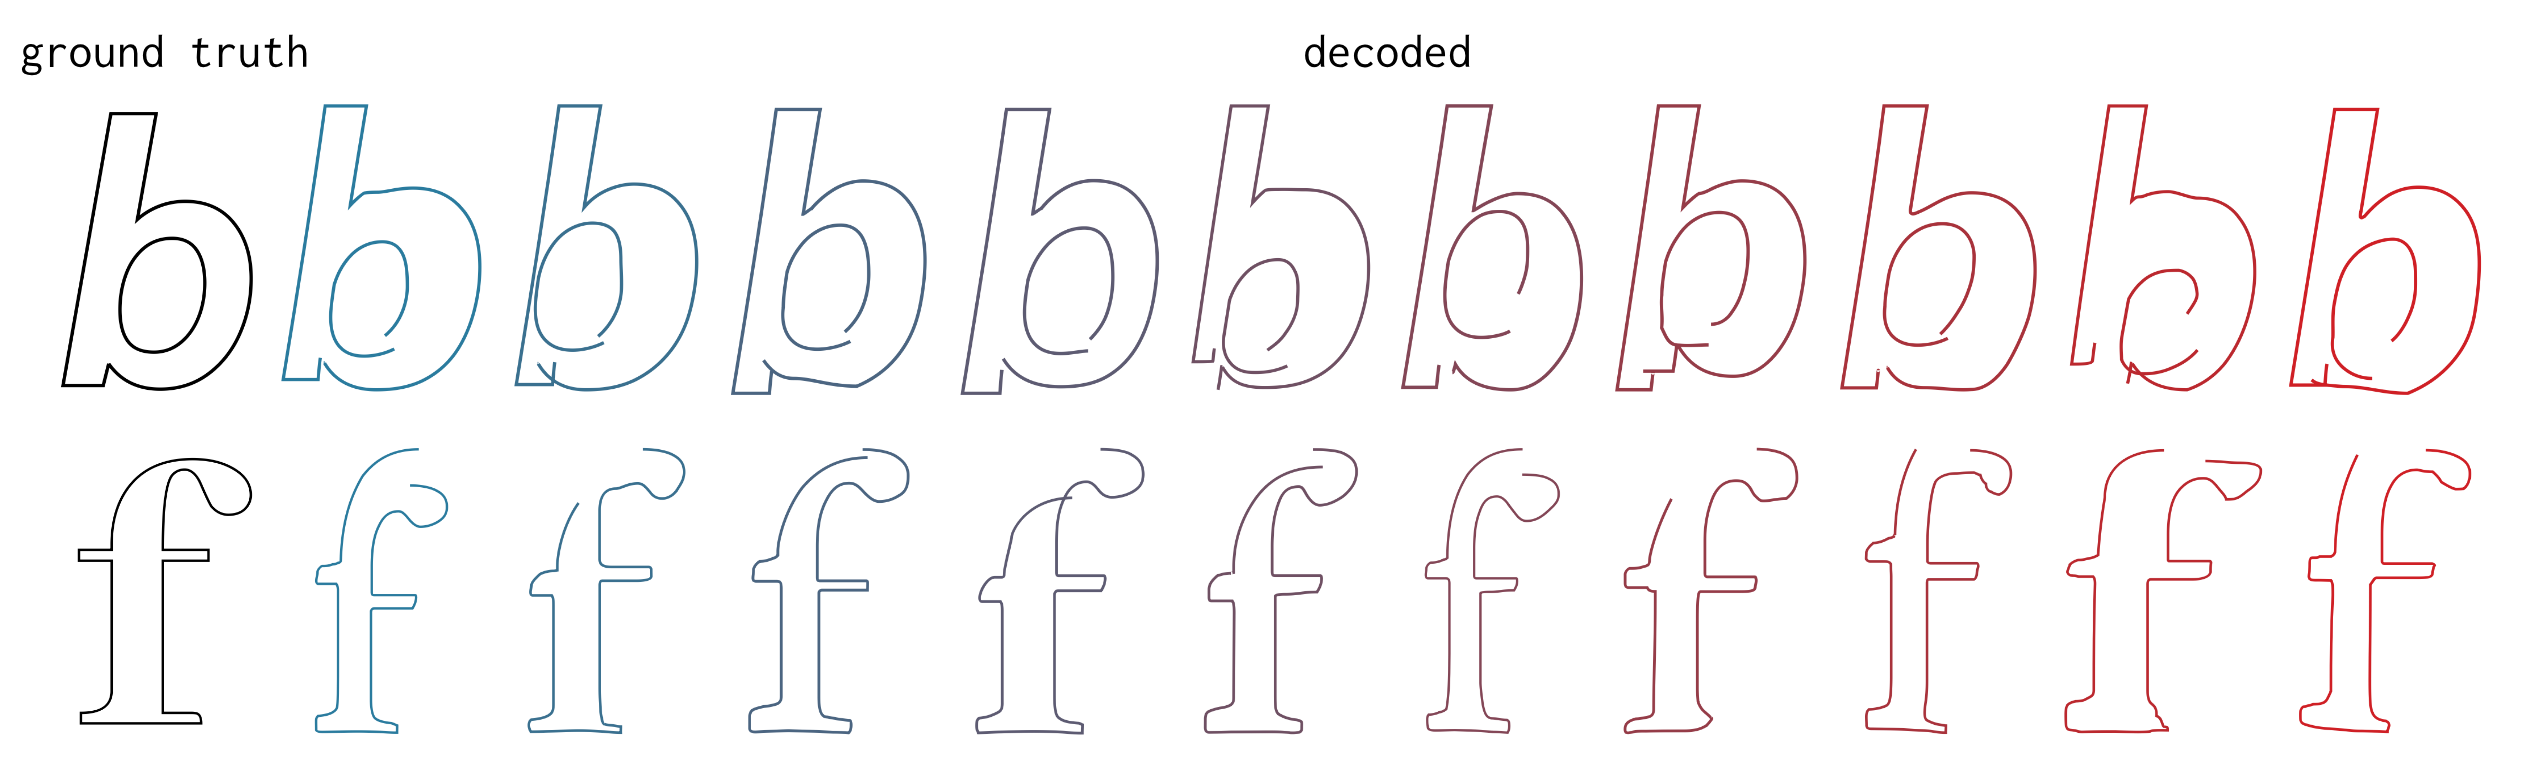
\includegraphics[width=\textwidth]{figures/temp_grid}
    \caption[The temperature grid for a conditionally generated glyph]
    {To demonstrate how temperature affects decoding, we decode the same latent vector at different temperature settings.
    At the far left, $\tau=0.1$, and at the far right, $\tau=1.0$, with $\tau$ increasing by 0.1 for every intermediate image.\label{fig:temp}}
\end{figure}

Figure~\ref{fig:fails} depicts common failure modes in conditional generation.
Because the model is drawing sequences of commands moving to relative points, it often struggles with closing the loop and returning to its original path start point.
Additionally, since we some font face styles are exceptionally rare, the model fails to learn how represent non-standard font styles.
\begin{figure}[h]
    \centering
	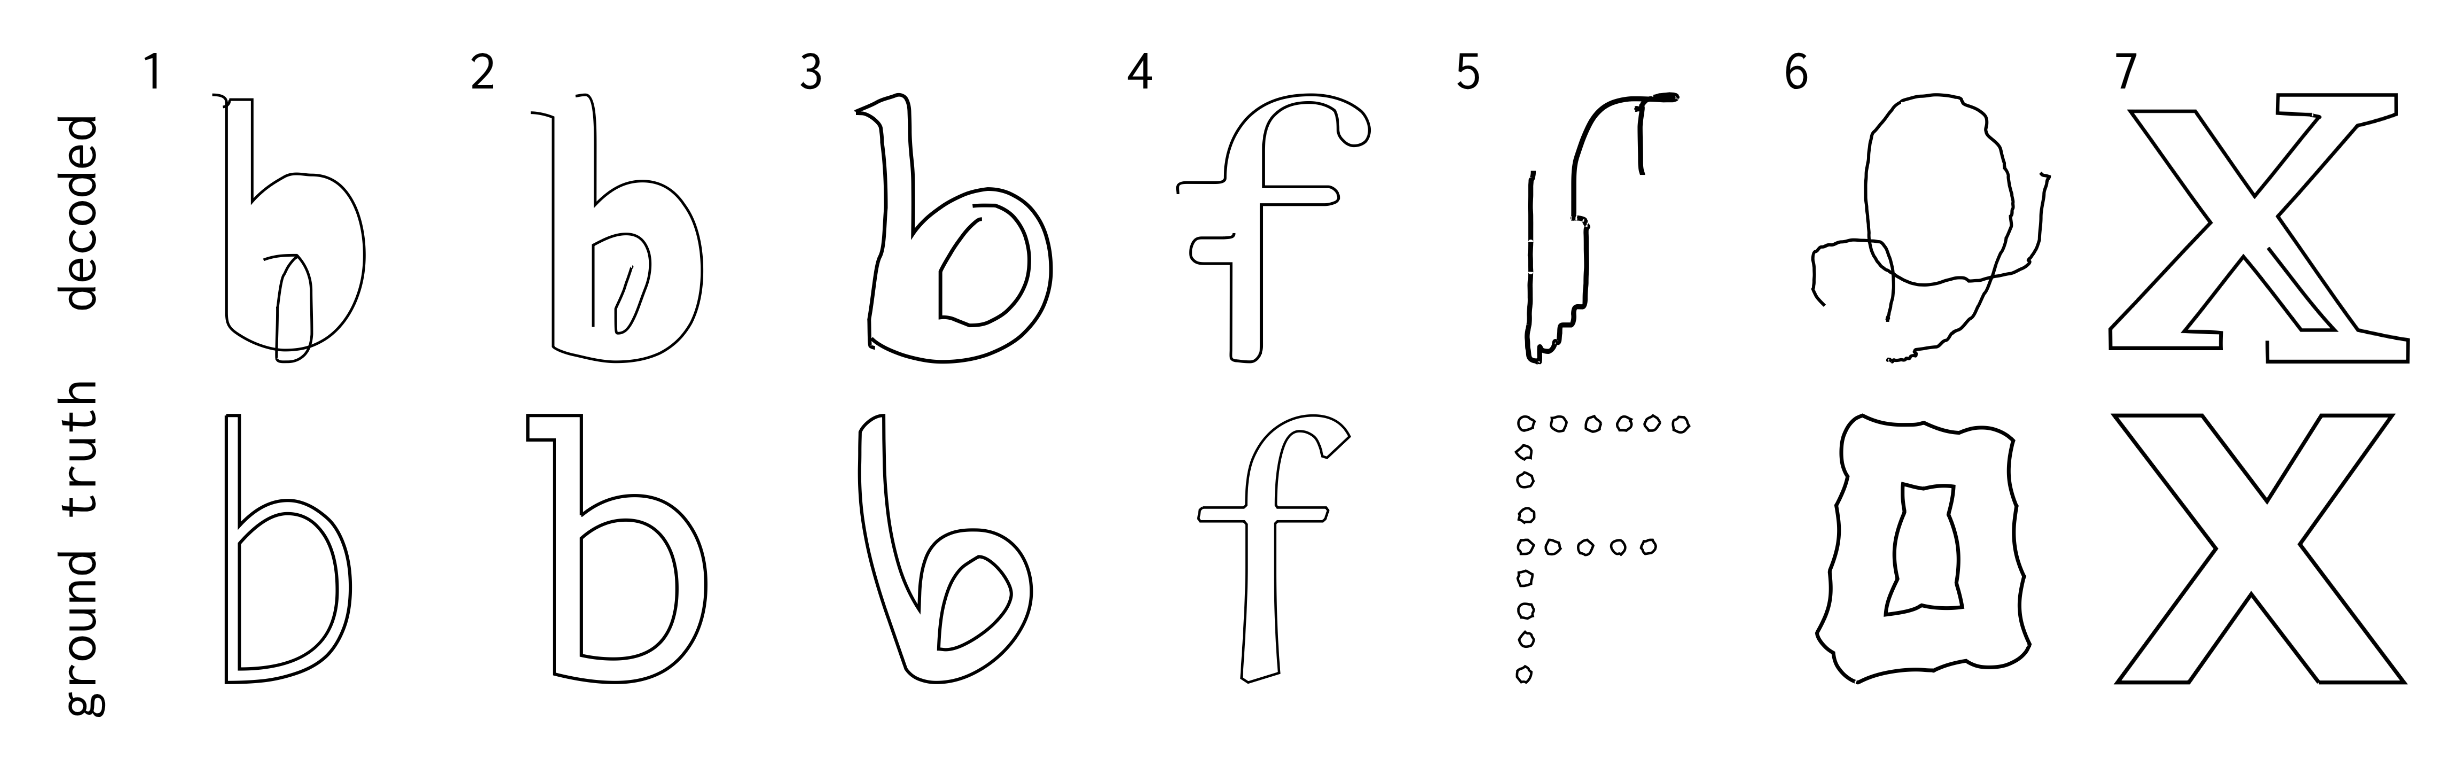
\includegraphics[width=\textwidth]{figures/fails}
    \caption[Common failure cases for conditional generation]
    {The model generally makes a set of common mistakes, as shown here.
    It struggles with positioning of disconnected components (1), closing paths (2, 4), understanding uncommon styles (3, 5, 6), and sometimes confuses styles (7).\label{fig:fails}}
\end{figure}

Finally, Figure~\ref{fig:uncond} demonstrates the creative ability of the model: generating unseen examples of a variety of styles.
Instead of encoding an input SVG and passing in the resulting latent vector into the decoder, we train the decoder separately to learn unconditional generation without a $z$ input.
\begin{figure}[h]
    \centering
	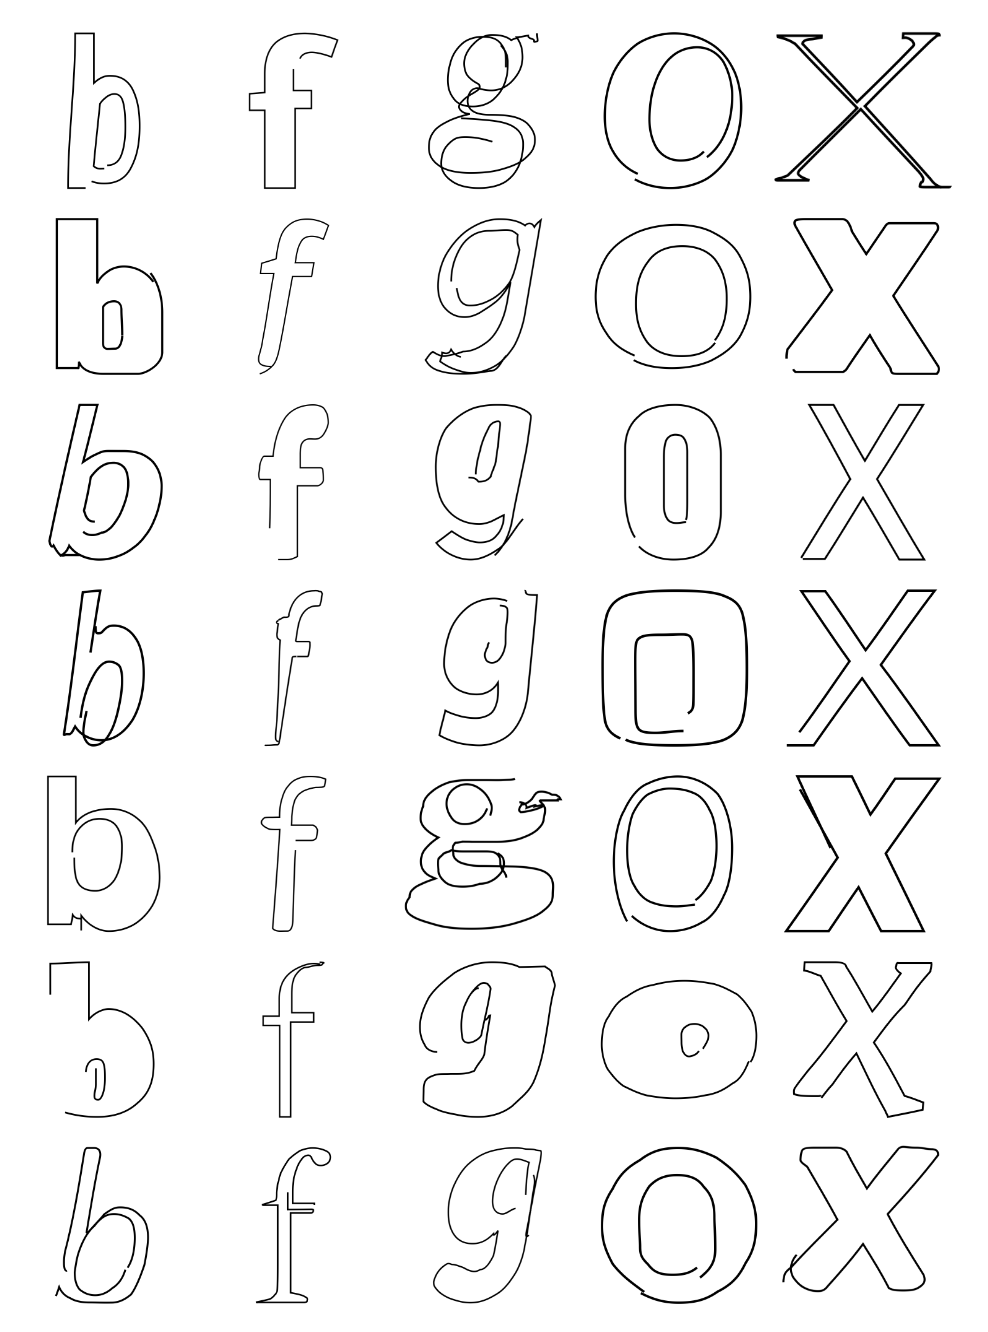
\includegraphics[width=\textwidth]{figures/uncond}
    \caption[Unconditional generation for the single-class model on letter glyphs]
    {We generate novel, unseen examples by training the decoder only without any latent variable input, feeding only the previously generated command into the decoder cells.
    Decoding here is done at $\tau=0.01$.
    \label{fig:uncond}}
\end{figure}

\chapter{Feature representation variability}\label{chap:feature-variation}
We find that alternative forms of this feature adaptation process have varying ``learnability'', as training variants of the transformed inputs with the same model architecture produces outputs of differing quality.

Some examples of variation are:
\begin{itemize}
\item \textbf{Absolute vs.\ relative coordinates}: are start, end, and control points represented in terms of their absolute position in the drawing or their relative displacement between each other?
\item \textbf{Coordinate system orientation}: if relative, do we specify displacement vectors in terms of the normal $\{(1, 0), (0, 1)\}$ basis, or do we transform their values such that they represent deviations from continuing in the same direction as the previous point?
\item \textbf{Pairwise coordinate choice}: if relative, between which points in the curves' coordinate parameters do we measure displacement?
\end{itemize}

\section{Evaluating feature encodings}\label{sec:eval-encs}
To investigate the effects of choices for the above questions, we train five models each with a different feature encoding for input and output drawings.
Code for generating each encoding can be found in Appendix~\ref{app:enc}.

\begin{table}[t]
\centering
\caption[Feature encoding variants]{The differences between the five feature representations used for the encoding efficacy experiment.
    Each feature encoding uses six dimensions for the cubic B\'ezier parameters (two for each point vector) and three for the pen state (pen up, pen down, end drawing).
    Note that \code{s} represents the start coordinates of the curve, \code{e} represents the end coordinates of the curve, \code{c1} represents the coordinates of the curve's first control point, and \code{c2} represents the coordinates of the curve's second control point.
    \code{disp(a, b)} indicates displacement between points \code{a} and \code{b}, and \code{rot(v)} indicates that vector \code{v} has been applied a transformation to rotate its coordinate axes to be in the direction of the previous vector in the encoding \TODO{wording?}.\label{tbl:features}}
\begin{tabularx}{\linewidth}{c X}
\toprule
    Encoding & Feature vector description \\ \midrule
    A & \code{disp(s, e), disp(s, c1), disp(s, c2), pen\_state}\\
    B & \code{disp(s, c1), disp(c1, c2), disp(c2, e), pen\_state}\\
    C & \code{disp(s, e), rot(disp(s, c1)), rot(disp(c2, e)), pen\_state}\\
    D & \code{e, rot(disp(s, c1)), rot(disp(c2, e)), pen\_state}\\
    E & \code{e, c1, c2, pen\_state}\\
\end{tabularx}
\end{table}

All models are trained using the same architecture as described in Section~\ref{sec:architecture}, for 125k steps.
To generate the differently encoded inputs, the same base dataset of SVGs for the glyph \textbf{b} in various font faces is transformed to produce a set of feature vectors for each representation in Table~\ref{tbl:features}.
The base dataset is then partitioned randomly into 1920 training examples, 240 validation examples, and 240 test examples.
SVGs whose total number of path commands is greater than 250 are pruned.
Graphs depicting loss during the training process can be found in Figure~\ref{appfig:train-encs}, and test costs for each selected model are reported in Tabel~\ref{apptbl:train-encs}.

\section{Results}
For each of the models, the model iteration with the best validation loss is selected for evaluation.

We evaluate results quantitatively by computing the Hausdorff similarity metric between each ground-truth image and a corresponding image conditionally generated by the model with $\tau = 0.3$, using the same method as described in Section~\ref{sec:quant-eval}.
Evaluation is run on a set of $N$ images for each encoding, and quantitative results can be found in Table~\ref{tbl:encoding-results}.

\begin{table}[t]
\centering
\caption[Quantitative results for evaluating feature encodings]
    {Modified Hausdorff distance for models trained on the \textbf{b} dataset with each encoding on a test set of $N$ images.\label{tbl:encoding-results}}
\begin{tabular}{c c c c c}
\toprule
    Encoding & Mean & Std.\ dev. & Kurtosis & $N$ \\ \midrule
    A & 28.7707 & 11.9332 & 1.3354 & 239 \\
    B & 15.4189 & 8.4912 & 3.1740 & 239 \\
    C & 24.8122 & 14.5086 & 17.9476 & 233 \\
    D & 15.9723 & 7.6134 & 0.9394 & 240 \\
    E & 16.7207 & 7.1926 & 0.8920 & 240 \\
\end{tabular}
\end{table}

Sample conditionally generated images can be found in Figure~\ref{fig:encodings}.
While encoding E maintains high image similarity as measured by the Hausdorff metric, its generated outputs tend to lack smooth curves and straight lines and are characterized instead by jagged, bite-mark shaped curves.
This demonstrates a potential shortcoming of our Hausdorff similarity metric: training a model on strokes' absolute positions seems to result in greater preservation of the original glyph shape but may make learning style properties more difficult.
Still, encodings B and D seem to result in the glyphs most visually similar to ground-truth glyphs and score relatively well on generated image similarity.
\TODO{We interpret this finding as suggesting that the model learns style and structure better when SVG data is encoded such that features represent displacement between adjacent control points---for example, start point and first control point, or second control point and end point.}

\begin{figure}[t]
    \centering
	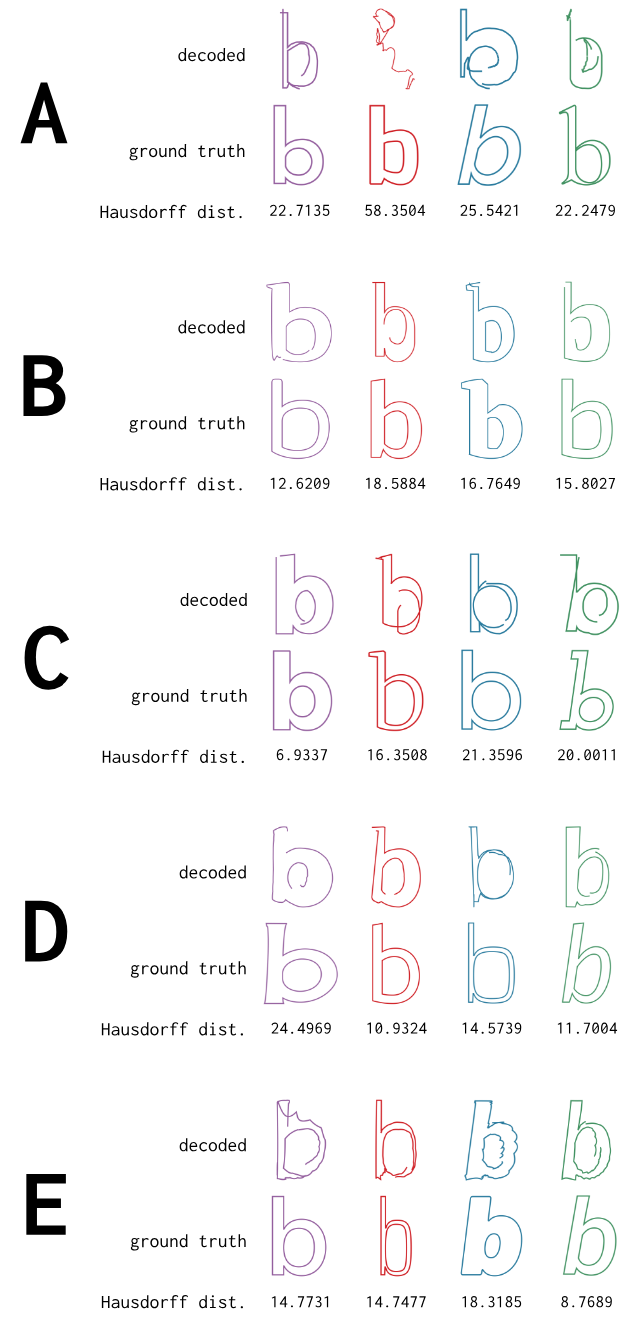
\includegraphics[height=0.8\textheight]{figures/encodings}
    \caption[Visual results of training the SVG model with different encodings]
    {Randomly sampled input-output pairs from the SVG models trained on the five encodings described in Table~\ref{tbl:features}.
    Decoded outputs were generated at temperature 0.3.
    Decoded outputs are found in the top row for each encoding, while ground truth inputs are in the bottom row.\label{fig:encodings}}
\end{figure}


\chapter{Style and content}\label{chap:style}
Although the model presented in Chapter~\ref{chap:architecture} learns to model SVGs from a single class, training on a multi-class dataset forces it to encode style and class together in its latent space.
Here, we investigate a modified architecture that explicitly encodes style and class separately.
We report experiment results and demonstrate applications in classification and style transfer.

\begin{figure}[h]
\centering
\caption[An overview of the SVG model architecture with explicit label encoding]
    {An overview of the SVG model architecture with explicit label encoding.
    The differences between this figure and Figure~\ref{fig:architecture} are highlighted in red.
\label{fig:label-arch}}
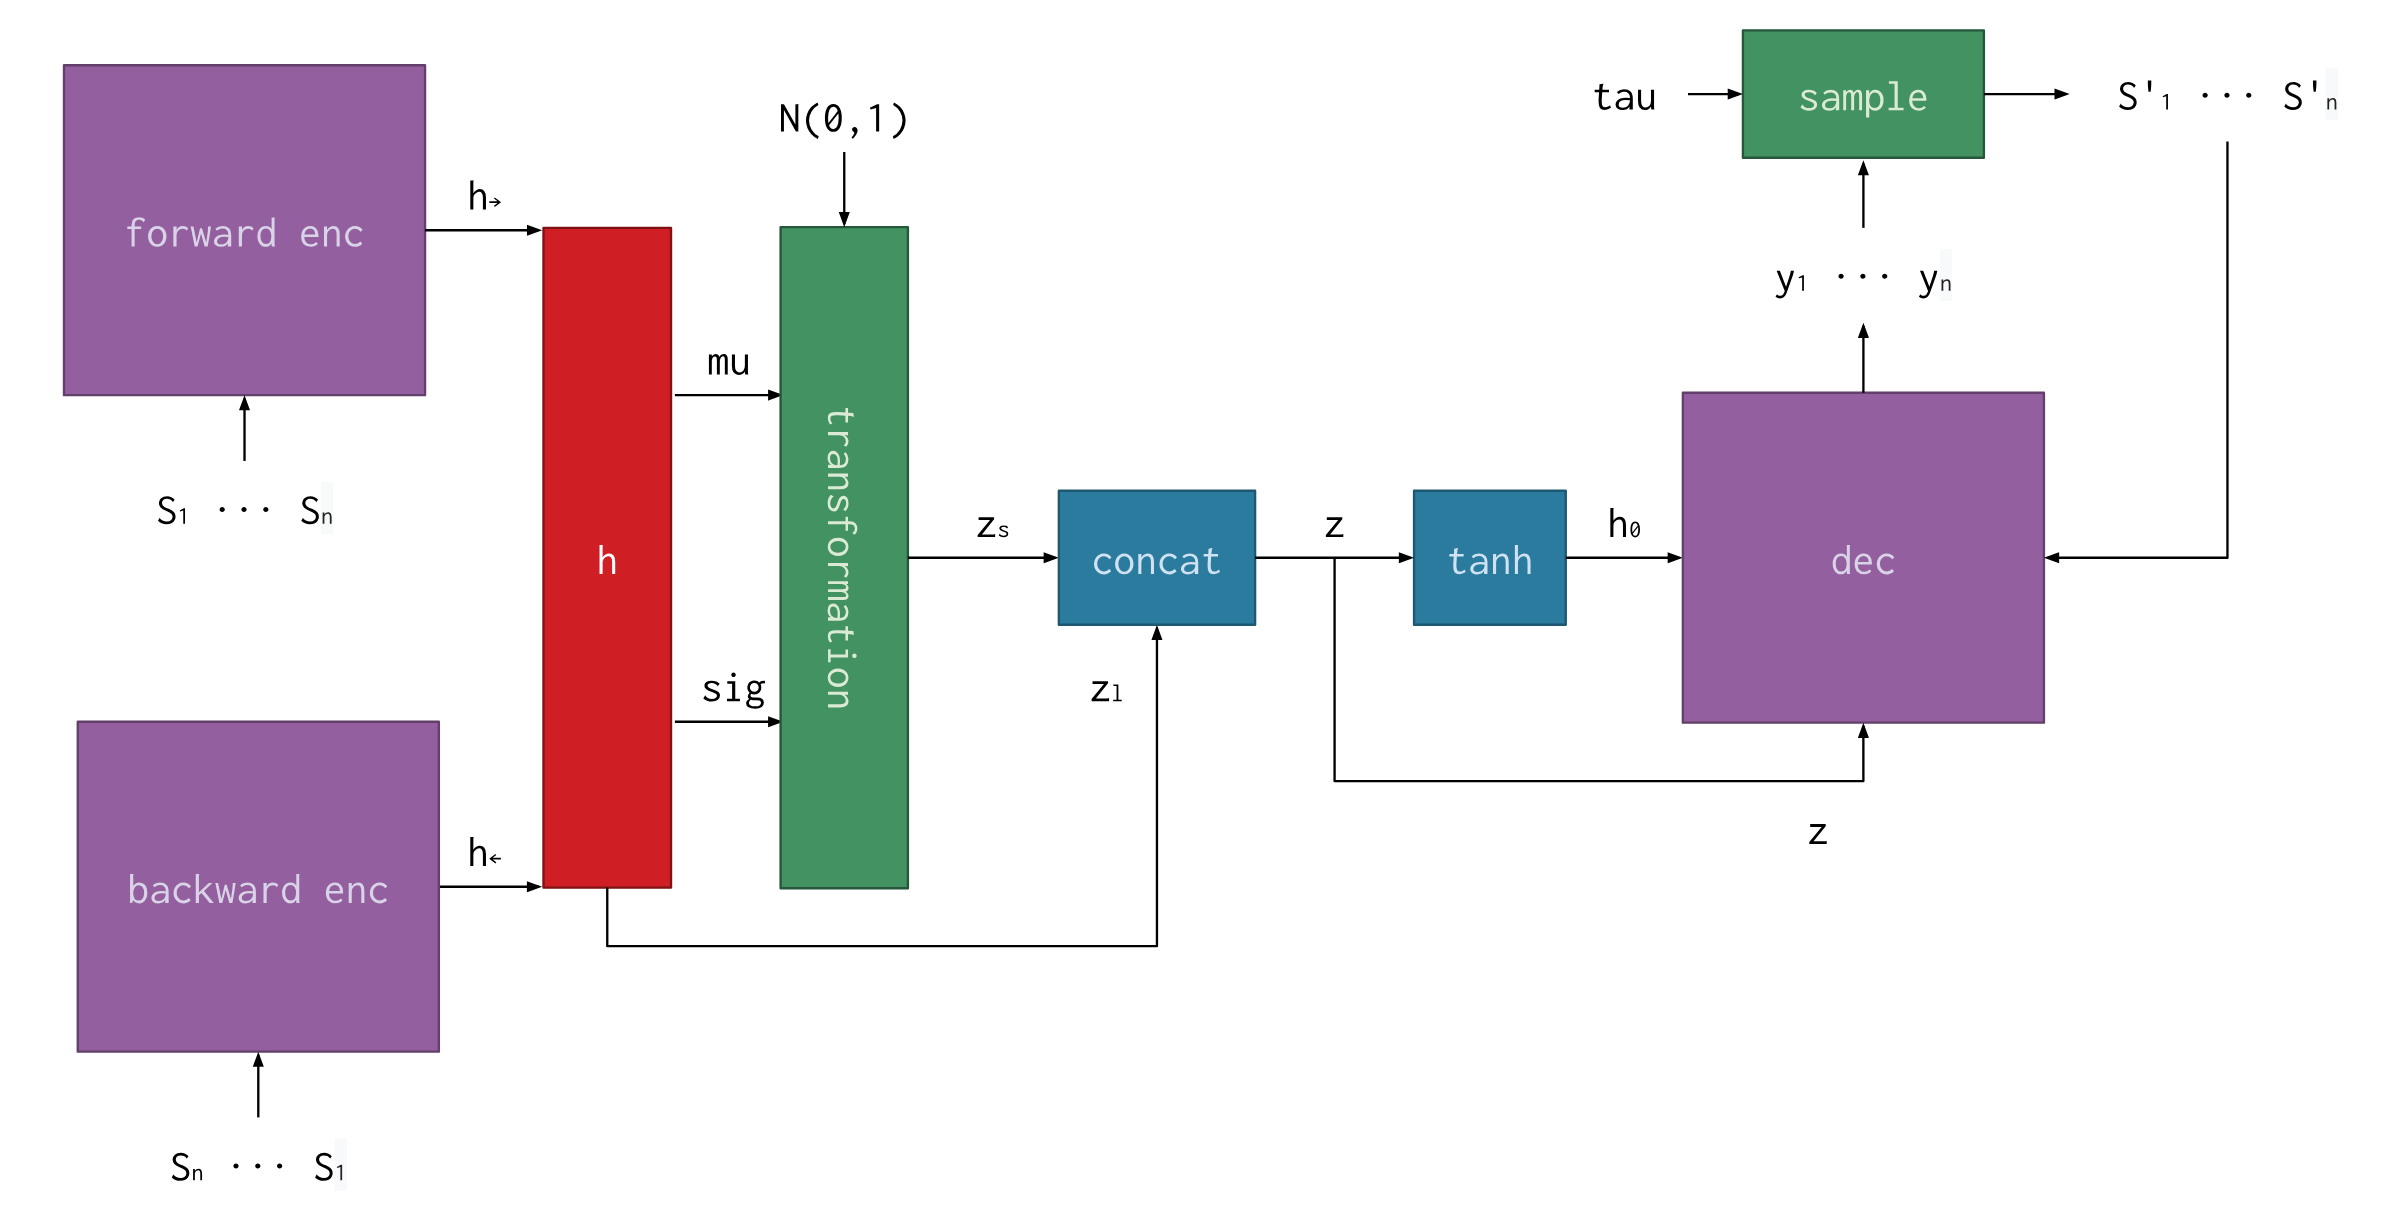
\includegraphics[width=\textwidth]{figures/label_architecture}
\end{figure}

\section{Model architecture}\label{sec:mod-arch}

The model presented originally transforms the final layer of the encoder RNN into $\mu$ and $\sigma$ vectors, which are then combined with random $\mathcal{N}(0,1)$ samples to form a latent space vector $z$.

We modify this architecture to also generate a label vector $z_l$ from the encoder's final layer that models a categorical distribution over input classes.
Assuming there are $n_c$ input classes and a latent space dimension of $n_z$, we adjust $\mu$ and $\sigma$ to be of dimension $n_z - n_c$, then perform the original transformation from $\mu$ and $\sigma$ to generate what we now denote as $z_s$.
We concatenate these two vectors, $z_l$ and $z_s$, to form $z$, which is then fed into the decoder as before.

Finally, we add another term in the cost function representing the log loss of the label prediction with the ground truth label (encoded as a $n_c$-dimensional one-hot vector).
With the ground truth label encoded as $(c_1, \cdots, c_{n_c})$, the log loss of label prediction is:

\begin{equation}
L_c = \sum_{i=1}^c c_i \log(z_{li})
\end{equation}

\section{Classifying experiment}
We perform an experiment comparing two models: one version of the original model and one version of the modified classification model.
To generate a multi-class dataset, we combine datasets for the digit glyphs (i.e. digits 0 through 9).
Input SVGs are encoded using encoding B as described in Chapter~\ref{chap:feature-variation}.
Overall, the resulting dataset has 20k training examples, 2.4k test examples, and 2.4k validation examples.

Both models were trained for 450k iterations with the same parameters as models described in Chapter~\ref{chap:training}, and details about training cost can be found in Appendix~\ref{app:train}.

\begin{figure}[h]
    \centering
	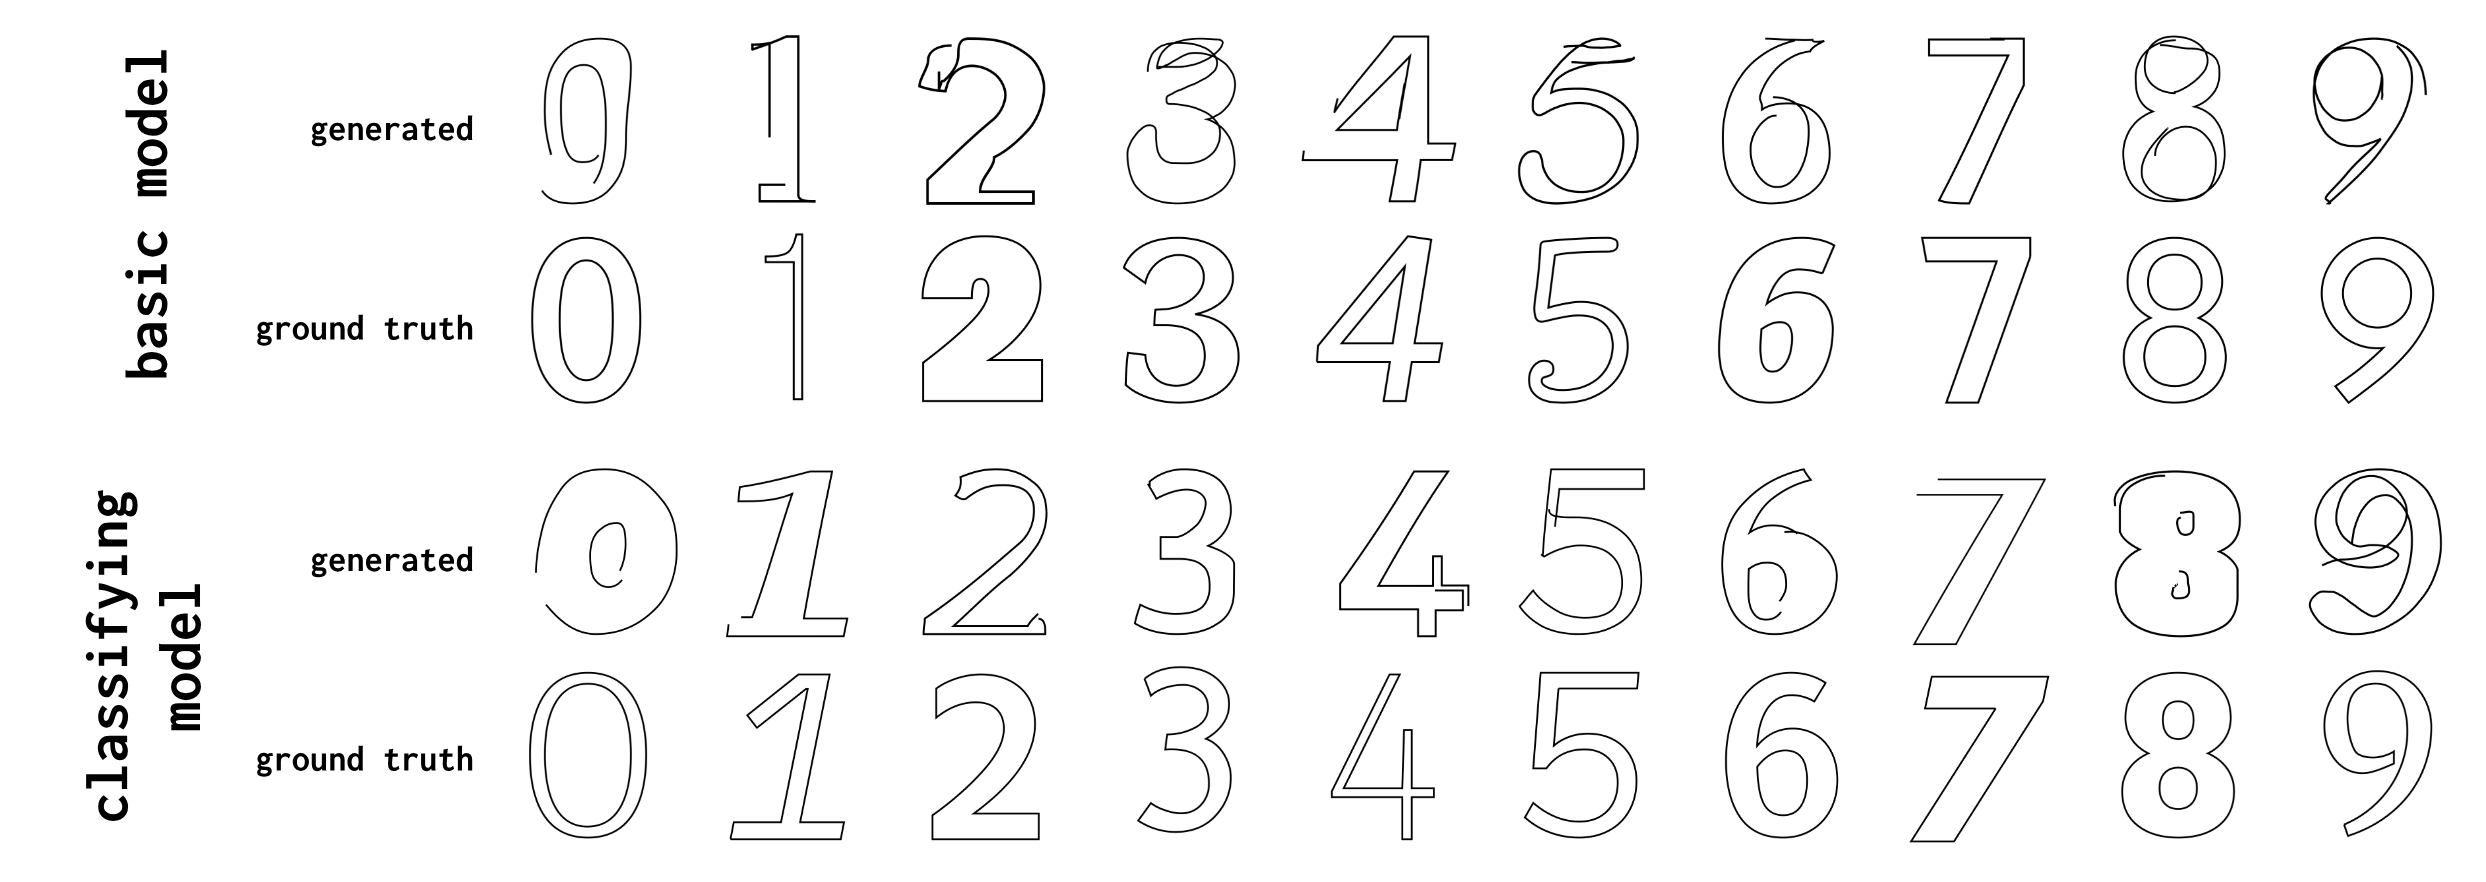
\includegraphics[width=\textwidth]{figures/digits}
    \caption[Visual results for the multi-class digits models]
    {Selected conditionally generated digits from the original model in Chapter~\ref{chap:architecture} and the modified model presented in Section~\ref{sec:mod-arch} trained on a multi-class digits dataset.\label{fig:class-results}}
\end{figure}

\section{Results}
In conditionally recreating input images, we find that the models are comparable, with the original model performing slightly better in quantitative evaluation. Selected decoded outputs from both models are shown in Figure~\ref{fig:class-results}.

\begin{table}[h]
\centering
\caption[Quantitative results for evaluating multi-class models]
    {Modified Hausdorff distance for models trained on the digit glyph dataset with each encoding on a test set of $N$ images.
    We include two baselines: one comparing every input digit image against random noise of the same image dimensions, and one comparing randomly selected pairs of input images.
    \label{tbl:class-results}}
\begin{tabular}{c c c c c}
\toprule
    Model & Mean & Std.\ dev. & Kurtosis & $N$ pairs \\ \midrule
    Original & 25.5308 & 10.5062 & 3.1082 & 2400 \\
    Modified & 26.6192 & 16.9867 & 15.8120 & 2326 \\ \midrule
    \multicolumn{5}{c}{Baselines} \\ \midrule
    Random noise & 183.6398 & 27.1631 & 1.8888 & 2400 \\
    Input pairs & 33.6121 & 13.3207 & 0.6291 & 500
\end{tabular}
\end{table}

We evaluate results quantitatively by computing the Hausdorff similarity metric between each ground truth test set image and a corresponding image conditionally generated by the model with $\tau = 0.1$, using the same method as described in Section~\ref{sec:quant-eval}.
Results are reported in Table~\ref{tbl:class-results}.
We also include a random noise baseline and an input pairs baseline.

\begin{table}[h]
\centering
\caption[Classification accuracy for the modified multi-class model]
    {Classification accuracy for the modified multi-class model.\label{tbl:class-acc}}
\begin{tabular}{c c}
\toprule
    Digit & Classification accuracy \\ \midrule
    0 & 82.08\% \\
    1 & 41.25\% \\
    2 & 92.91\% \\
    3 & 97.08\% \\
    4 & 49.16\% \\
    5 & 56.66\% \\
    6 & 61.25\% \\
    7 & 80.83\% \\
    8 & 95.83\% \\
    9 & 88.33\%
\end{tabular}
\end{table}

Finally, we report the classification accuracy from the modified model, generated by comparing the highest probability predicted class to the ground truth class.
The modified model has an overall classification accuracy of 74.54\%, with accuracy rates per class reported in Table~\ref{tbl:class-acc}.

One factor that may partially explain the classifying model's lack of improvement in generating conditional images over the basic model is the reduced latent vector size.
Both models set $n_z$ to be 128, but the basic model is able to use the entire latent vector to encode the input drawing, while the classifying model must reserve 10 dimensions for the digit class vector.
Future work can explore this hypothesis as well as experiment with other adjustments to the model architecture to further improve performance.

\section{Style transfer}
We verify that the class encoding is used by the decoder by manually substituting out the portion of $z$ corresponding to $z_c$ with a different class encoding.
Although we did not quantitatively evaluate these results, we report visual results for more common font styles in Figure~\ref{fig:style-trans}. 

\begin{figure}[h]
    \centering
	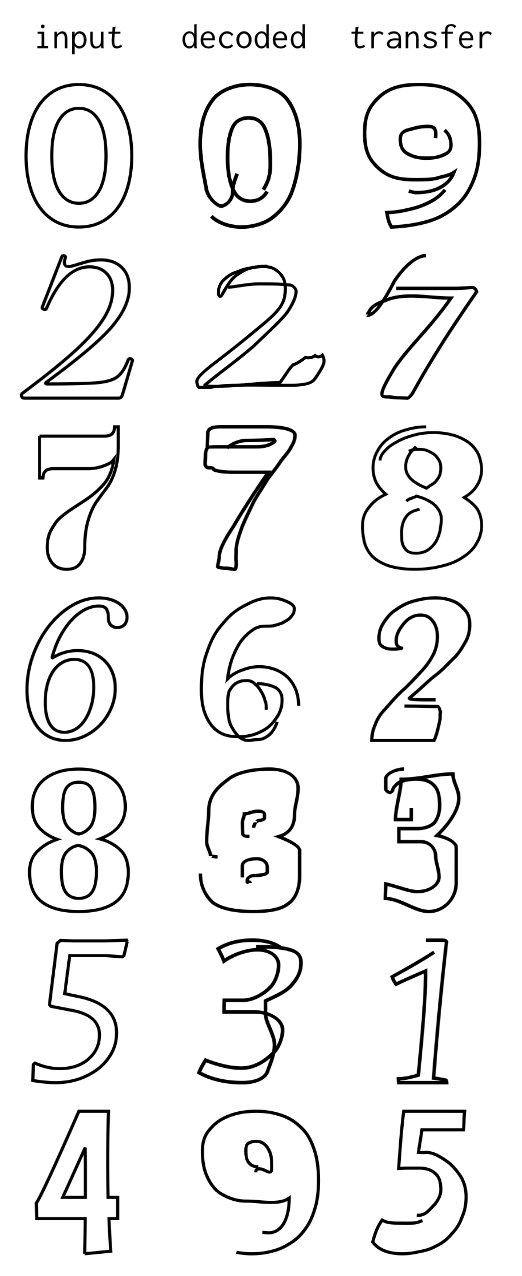
\includegraphics[height=0.9\textheight]{figures/style_trans}
    \caption[Examples of style transfer using the classifying model]
    {Examples of style transfer using the classifying model.
    Outputs were decoded at $\tau=0.1$.
    In the last two rows, the model misclassified the input 5 as 3 and the input 4 as 9, resulting in the incorrect decoded output.
    \label{fig:style-trans}}
\end{figure}

\chapter{Conclusion}

\appendix
\TODO{put appendix back in}
% \chapter{Arc conversion}\label{app:algs}
Our method for approximating SVG arc segments with cubic B\'ezier curves is as follows:
\begin{enumerate}
    \item Extract the arc parameters: start coordinates, end coordinates, ellipse major and minor radii, rotation angle from $x$ and $y$ axes, large arc flag, and sweep flag. 
    \item Transform ellipse into unit circle by rotating, scaling, and translating, and save those transformation factors.
    \item Find the arc angle from the transformed start point to end point on the unit circle.
    \item If needed, split the arc into segments, each covering an angle less than $90^\circ$.
    \item Approximate each segment angle's arc on a unit circle such that the distance from the circle center to the arc along the angle bisector of the arc is equal to the radius, defining cubic B\'ezier control points.
	\item Invert the transformation above to convert arcs along the unit circle back to the elliptical arc, transforming the generated control points accordingly.
	\item Use these transformed control points to parameterize the output cubic B\'ezier curve.
\end{enumerate}

% \chapter{Dataset statistics}\label{app:data}
\begin{figure}[h]
\caption[Dataset statistics for other glyphs]
{Dataset statistics for the remaining glyphs on which our model was trained across all 2552 font faces in the Google Fonts dataset.\label{fig:stats-rem}}
\centering
\subcaptionbox*{}
{\begin{tikzpicture}
\begin{axis}[
 	xlabel={feature vector count},
	ylabel={number of ``f'' glyphs},
	width=0.45\textwidth,
    ybar,
    ymin=0
]
\addplot [
	fill=color1,
	fill opacity=0.4,
    hist={
        bins=7,
        data min=0.5,
        data max=300
    }   
] table [y index=0] {data/f_points_stats.csv};
\end{axis}
\end{tikzpicture}
}
\subcaptionbox*{}
{\begin{tikzpicture}
\begin{axis}[
 	xlabel={command type count},
	ylabel={number of ``f'' glyphs},
	width=0.45\textwidth,
    ybar,
    ymin=0
]
\addplot [
	fill=color2,
	fill opacity=0.4,
    hist={
        bins=7,
        data min=0.5,
        data max=100
    }   
] table [y index=0] {data/f_line_count.csv};
\addplot [
	fill=color3,
	fill opacity=0.4,
    hist={
        bins=7,
        data min=0.5,
        data max=100
    }   
] table [y index=0] {data/f_quad_count.csv};
\addlegendentry{\code{line}}
\addlegendentry{\code{quad}}
\end{axis}
\end{tikzpicture}
}

\subcaptionbox*{}
{\begin{tikzpicture}
\begin{axis}[
 	xlabel={feature vector count},
	ylabel={number of ``g'' glyphs},
	width=0.45\textwidth,
    ybar,
    ymin=0
]
\addplot [
	fill=color1,
	fill opacity=0.4,
    hist={
        bins=7,
        data min=0.5,
        data max=300
    }   
] table [y index=0] {data/g_points_stats.csv};
\end{axis}
\end{tikzpicture}
}
\subcaptionbox*{}
{\begin{tikzpicture}
\begin{axis}[
 	xlabel={command type count},
	ylabel={number of ``g'' glyphs},
	width=0.45\textwidth,
    ybar,
    ymin=0
]
\addplot [
	fill=color2,
	fill opacity=0.4,
    hist={
        bins=7,
        data min=0.5,
        data max=100
    }   
] table [y index=0] {data/g_line_count.csv};
\addplot [
	fill=color3,
	fill opacity=0.4,
    hist={
        bins=7,
        data min=0.5,
        data max=100
    }   
] table [y index=0] {data/g_quad_count.csv};
\addlegendentry{\code{line}}
\addlegendentry{\code{quad}}
\end{axis}
\end{tikzpicture}
}
\end{figure}

\begin{figure}[h]
\centering
\subcaptionbox*{}
{\begin{tikzpicture}
\begin{axis}[
 	xlabel={feature vector count},
	ylabel={number of ``o'' glyphs},
	width=0.45\textwidth,
    ybar,
    ymin=0
]
\addplot [
	fill=color1,
	fill opacity=0.4,
    hist={
        bins=7,
        data min=0.5,
        data max=300
    }   
] table [y index=0] {data/o_points_stats.csv};
\end{axis}
\end{tikzpicture}
}
\subcaptionbox*{}
{\begin{tikzpicture}
\begin{axis}[
 	xlabel={command type count},
	ylabel={number of ``o'' glyphs},
	width=0.45\textwidth,
    ybar,
    ymin=0
]
\addplot [
	fill=color2,
	fill opacity=0.4,
    hist={
        bins=7,
        data min=0.5,
        data max=100
    }   
] table [y index=0] {data/o_line_count.csv};
\addplot [
	fill=color3,
	fill opacity=0.4,
    hist={
        bins=7,
        data min=0.5,
        data max=100
    }   
] table [y index=0] {data/o_quad_count.csv};
\addlegendentry{\code{line}}
\addlegendentry{\code{quad}}
\end{axis}
\end{tikzpicture}
}

\subcaptionbox*{}
{\begin{tikzpicture}
\begin{axis}[
 	xlabel={feature vector count},
	ylabel={number of ``x'' glyphs},
	width=0.45\textwidth,
    ybar,
    ymin=0
]
\addplot [
	fill=color1,
	fill opacity=0.4,
    hist={
        bins=7,
        data min=0.5,
        data max=300
    }   
] table [y index=0] {data/x_points_stats.csv};
\end{axis}
\end{tikzpicture}
}
\subcaptionbox*{}
{\begin{tikzpicture}
\begin{axis}[
 	xlabel={command type count},
	ylabel={number of ``x'' glyphs},
	width=0.45\textwidth,
    ybar,
    ymin=0
]
\addplot [
	fill=color2,
	fill opacity=0.4,
    hist={
        bins=7,
        data min=0.5,
        data max=100
    }   
] table [y index=0] {data/x_line_count.csv};
\addplot [
	fill=color3,
	fill opacity=0.4,
    hist={
        bins=7,
        data min=0.5,
        data max=100
    }   
] table [y index=0] {data/x_quad_count.csv};
\addlegendentry{\code{line}}
\addlegendentry{\code{quad}}
\end{axis}
\end{tikzpicture}
}

\subcaptionbox*{}
{\begin{tikzpicture}
\begin{axis}[
 	xlabel={feature vector count},
	ylabel={number of ``0'' glyphs},
	width=0.45\textwidth,
    ybar,
    ymin=0
]
\addplot [
	fill=color1,
	fill opacity=0.4,
    hist={
        bins=7,
        data min=0.5,
        data max=300
    }   
] table [y index=0] {data/zero_points_stats.csv};
\end{axis}
\end{tikzpicture}
}
\subcaptionbox*{}
{\begin{tikzpicture}
\begin{axis}[
 	xlabel={command type count},
	ylabel={number of ``0'' glyphs},
	width=0.45\textwidth,
    ybar,
    ymin=0
]
\addplot [
	fill=color2,
	fill opacity=0.4,
    hist={
        bins=7,
        data min=0.5,
        data max=100
    }   
] table [y index=0] {data/zero_line_count.csv};
\addplot [
	fill=color3,
	fill opacity=0.4,
    hist={
        bins=7,
        data min=0.5,
        data max=100
    }   
] table [y index=0] {data/zero_quad_count.csv};
\addlegendentry{\code{line}}
\addlegendentry{\code{quad}}
\end{axis}
\end{tikzpicture}
}
\end{figure}

\begin{figure}[h]
\centering
\subcaptionbox*{}
{\begin{tikzpicture}
\begin{axis}[
 	xlabel={feature vector count},
	ylabel={number of ``1'' glyphs},
	width=0.45\textwidth,
    ybar,
    ymin=0
]
\addplot [
	fill=color1,
	fill opacity=0.4,
    hist={
        bins=7,
        data min=0.5,
        data max=300
    }   
] table [y index=0] {data/one_points_stats.csv};
\end{axis}
\end{tikzpicture}
}
\subcaptionbox*{}
{\begin{tikzpicture}
\begin{axis}[
 	xlabel={command type count},
	ylabel={number of ``1'' glyphs},
	width=0.45\textwidth,
    ybar,
    ymin=0
]
\addplot [
	fill=color2,
	fill opacity=0.4,
    hist={
        bins=7,
        data min=0.5,
        data max=100
    }   
] table [y index=0] {data/one_line_count.csv};
\addplot [
	fill=color3,
	fill opacity=0.4,
    hist={
        bins=7,
        data min=0.5,
        data max=100
    }   
] table [y index=0] {data/one_quad_count.csv};
\addlegendentry{\code{line}}
\addlegendentry{\code{quad}}
\end{axis}
\end{tikzpicture}
}

\subcaptionbox*{}
{\begin{tikzpicture}
\begin{axis}[
 	xlabel={feature vector count},
	ylabel={number of ``2'' glyphs},
	width=0.45\textwidth,
    ybar,
    ymin=0
]
\addplot [
	fill=color1,
	fill opacity=0.4,
    hist={
        bins=7,
        data min=0.5,
        data max=300
    }   
] table [y index=0] {data/two_points_stats.csv};
\end{axis}
\end{tikzpicture}
}
\subcaptionbox*{}
{\begin{tikzpicture}
\begin{axis}[
 	xlabel={command type count},
	ylabel={number of ``2'' glyphs},
	width=0.45\textwidth,
    ybar,
    ymin=0
]
\addplot [
	fill=color2,
	fill opacity=0.4,
    hist={
        bins=7,
        data min=0.5,
        data max=100
    }   
] table [y index=0] {data/two_line_count.csv};
\addplot [
	fill=color3,
	fill opacity=0.4,
    hist={
        bins=7,
        data min=0.5,
        data max=100
    }   
] table [y index=0] {data/two_quad_count.csv};
\addlegendentry{\code{line}}
\addlegendentry{\code{quad}}
\end{axis}
\end{tikzpicture}
}

\subcaptionbox*{}
{\begin{tikzpicture}
\begin{axis}[
 	xlabel={feature vector count},
	ylabel={number of ``3'' glyphs},
	width=0.45\textwidth,
    ybar,
    ymin=0
]
\addplot [
	fill=color1,
	fill opacity=0.4,
    hist={
        bins=7,
        data min=0.5,
        data max=300
    }   
] table [y index=0] {data/three_points_stats.csv};
\end{axis}
\end{tikzpicture}
}
\subcaptionbox*{}
{\begin{tikzpicture}
\begin{axis}[
 	xlabel={command type count},
	ylabel={number of ``3'' glyphs},
	width=0.45\textwidth,
    ybar,
    ymin=0
]
\addplot [
	fill=color2,
	fill opacity=0.4,
    hist={
        bins=7,
        data min=0.5,
        data max=100
    }   
] table [y index=0] {data/three_line_count.csv};
\addplot [
	fill=color3,
	fill opacity=0.4,
    hist={
        bins=7,
        data min=0.5,
        data max=100
    }   
] table [y index=0] {data/three_quad_count.csv};
\addlegendentry{\code{line}}
\addlegendentry{\code{quad}}
\end{axis}
\end{tikzpicture}
}
\end{figure}

\begin{figure}[h]
\centering
\subcaptionbox*{}
{\begin{tikzpicture}
\begin{axis}[
 	xlabel={feature vector count},
	ylabel={number of ``4'' glyphs},
	width=0.45\textwidth,
    ybar,
    ymin=0
]
\addplot [
	fill=color1,
	fill opacity=0.4,
    hist={
        bins=7,
        data min=0.5,
        data max=300
    }   
] table [y index=0] {data/four_points_stats.csv};
\end{axis}
\end{tikzpicture}
}
\subcaptionbox*{}
{\begin{tikzpicture}
\begin{axis}[
 	xlabel={command type count},
	ylabel={number of ``4'' glyphs},
	width=0.45\textwidth,
    ybar,
    ymin=0
]
\addplot [
	fill=color2,
	fill opacity=0.4,
    hist={
        bins=7,
        data min=0.5,
        data max=100
    }   
] table [y index=0] {data/four_line_count.csv};
\addplot [
	fill=color3,
	fill opacity=0.4,
    hist={
        bins=7,
        data min=0.5,
        data max=100
    }   
] table [y index=0] {data/four_quad_count.csv};
\addlegendentry{\code{line}}
\addlegendentry{\code{quad}}
\end{axis}
\end{tikzpicture}
}

\subcaptionbox*{}
{\begin{tikzpicture}
\begin{axis}[
 	xlabel={feature vector count},
	ylabel={number of ``5'' glyphs},
	width=0.45\textwidth,
    ybar,
    ymin=0
]
\addplot [
	fill=color1,
	fill opacity=0.4,
    hist={
        bins=7,
        data min=0.5,
        data max=300
    }   
] table [y index=0] {data/five_points_stats.csv};
\end{axis}
\end{tikzpicture}
}
\subcaptionbox*{}
{\begin{tikzpicture}
\begin{axis}[
 	xlabel={command type count},
	ylabel={number of ``5'' glyphs},
	width=0.45\textwidth,
    ybar,
    ymin=0
]
\addplot [
	fill=color2,
	fill opacity=0.4,
    hist={
        bins=7,
        data min=0.5,
        data max=100
    }   
] table [y index=0] {data/five_line_count.csv};
\addplot [
	fill=color3,
	fill opacity=0.4,
    hist={
        bins=7,
        data min=0.5,
        data max=100
    }   
] table [y index=0] {data/five_quad_count.csv};
\addlegendentry{\code{line}}
\addlegendentry{\code{quad}}
\end{axis}
\end{tikzpicture}
}

\subcaptionbox*{}
{\begin{tikzpicture}
\begin{axis}[
 	xlabel={feature vector count},
	ylabel={number of ``6'' glyphs},
	width=0.45\textwidth,
    ybar,
    ymin=0
]
\addplot [
	fill=color1,
	fill opacity=0.4,
    hist={
        bins=7,
        data min=0.5,
        data max=300
    }   
] table [y index=0] {data/six_points_stats.csv};
\end{axis}
\end{tikzpicture}
}
\subcaptionbox*{}
{\begin{tikzpicture}
\begin{axis}[
 	xlabel={command type count},
	ylabel={number of ``6'' glyphs},
	width=0.45\textwidth,
    ybar,
    ymin=0
]
\addplot [
	fill=color2,
	fill opacity=0.4,
    hist={
        bins=7,
        data min=0.5,
        data max=100
    }   
] table [y index=0] {data/six_line_count.csv};
\addplot [
	fill=color3,
	fill opacity=0.4,
    hist={
        bins=7,
        data min=0.5,
        data max=100
    }   
] table [y index=0] {data/six_quad_count.csv};
\addlegendentry{\code{line}}
\addlegendentry{\code{quad}}
\end{axis}
\end{tikzpicture}
}
\end{figure}

\begin{figure}[h]
\centering
\subcaptionbox*{}
{\begin{tikzpicture}
\begin{axis}[
 	xlabel={feature vector count},
	ylabel={number of ``7'' glyphs},
	width=0.45\textwidth,
    ybar,
    ymin=0
]
\addplot [
	fill=color1,
	fill opacity=0.4,
    hist={
        bins=7,
        data min=0.5,
        data max=300
    }   
] table [y index=0] {data/seven_points_stats.csv};
\end{axis}
\end{tikzpicture}
}
\subcaptionbox*{}
{\begin{tikzpicture}
\begin{axis}[
 	xlabel={command type count},
	ylabel={number of ``7'' glyphs},
	width=0.45\textwidth,
    ybar,
    ymin=0
]
\addplot [
	fill=color2,
	fill opacity=0.4,
    hist={
        bins=7,
        data min=0.5,
        data max=100
    }   
] table [y index=0] {data/seven_line_count.csv};
\addplot [
	fill=color3,
	fill opacity=0.4,
    hist={
        bins=7,
        data min=0.5,
        data max=100
    }   
] table [y index=0] {data/seven_quad_count.csv};
\addlegendentry{\code{line}}
\addlegendentry{\code{quad}}
\end{axis}
\end{tikzpicture}
}

\subcaptionbox*{}
{\begin{tikzpicture}
\begin{axis}[
 	xlabel={feature vector count},
	ylabel={number of ``8'' glyphs},
	width=0.45\textwidth,
    ybar,
    ymin=0
]
\addplot [
	fill=color1,
	fill opacity=0.4,
    hist={
        bins=7,
        data min=0.5,
        data max=300
    }   
] table [y index=0] {data/eight_points_stats.csv};
\end{axis}
\end{tikzpicture}
}
\subcaptionbox*{}
{\begin{tikzpicture}
\begin{axis}[
 	xlabel={command type count},
	ylabel={number of ``8'' glyphs},
	width=0.45\textwidth,
    ybar,
    ymin=0
]
\addplot [
	fill=color2,
	fill opacity=0.4,
    hist={
        bins=7,
        data min=0.5,
        data max=100
    }   
] table [y index=0] {data/eight_line_count.csv};
\addplot [
	fill=color3,
	fill opacity=0.4,
    hist={
        bins=7,
        data min=0.5,
        data max=100
    }   
] table [y index=0] {data/eight_quad_count.csv};
\addlegendentry{\code{line}}
\addlegendentry{\code{quad}}
\end{axis}
\end{tikzpicture}
}

\subcaptionbox*{}
{\begin{tikzpicture}
\begin{axis}[
 	xlabel={feature vector count},
	ylabel={number of ``9'' glyphs},
	width=0.45\textwidth,
    ybar,
    ymin=0
]
\addplot [
	fill=color1,
	fill opacity=0.4,
    hist={
        bins=7,
        data min=0.5,
        data max=300
    }   
] table [y index=0] {data/nine_points_stats.csv};
\end{axis}
\end{tikzpicture}
}
\subcaptionbox*{}
{\begin{tikzpicture}
\begin{axis}[
 	xlabel={command type count},
	ylabel={number of ``9'' glyphs},
	width=0.45\textwidth,
    ybar,
    ymin=0
]
\addplot [
	fill=color2,
	fill opacity=0.4,
    hist={
        bins=7,
        data min=0.5,
        data max=100
    }   
] table [y index=0] {data/nine_line_count.csv};
\addplot [
	fill=color3,
	fill opacity=0.4,
    hist={
        bins=7,
        data min=0.5,
        data max=100
    }   
] table [y index=0] {data/nine_quad_count.csv};
\addlegendentry{\code{line}}
\addlegendentry{\code{quad}}
\end{axis}
\end{tikzpicture}
}
\end{figure}


% \chapter{Training}\label{app:train}

\begin{table}[h]
\centering
    \caption[Training results for the single-glyph models]{Training results and validation costs for single-glyph models described in Chapter~\ref{chap:training}.
    Models were run against the validation set every 5k iterations, and the model with the best validation cost is reported.
    We also report the overall, KL, and reconstruction losses of the best-performing model for each encoding on the test set.
    \label{apptbl:train-models}}
\begin{tabularx}{\textwidth}{c c X c c c}
\toprule
    Glyph & Iterations trained & Best model iteration & Test cost & Test KL loss & Test R loss \\ \midrule
    \textbf{b} & 610k & 105k & -1.830 & 0.5585 & -1.836 \\
    \textbf{f} & 573k & 205k & -1.669 & 0.4151 & -1.673 \\
    \textbf{g} & 471k & 65k & -2.075 & 0.7274 & -2.082 \\
    \textbf{o} & 438k & 280k & -1.733 & 0.2448 & -1.736 \\
    \textbf{x} & 566k & 60k & -1.055 & 0.2946 & -1.058 \\
\end{tabularx}
\end{table}

\begin{figure}[h]
\centering
\caption[Training and validation costs for the single-glyph models]
{Training and validation costs for the models trained in Chapter~\ref{chap:training}.\label{appfig:train-models}}
\subcaptionbox{Glyph \textbf{b}}
{
    \begin{tikzpicture}
        \begin{axis}[scale only axis,
                     width=0.35\textwidth,
                     xlabel={step},
                     ylabel={training cost},
                     label style={font=\scriptsize},
                     tick label style={font=\tiny},
                     x label style={at={(axis description cs:0.5,-0.1)},anchor=north},
                     y label style={at={(axis description cs:-0.1,.5)},anchor=south},]
          \addplot table [x=Step, y=Value, col sep=comma] {data/font_b_train_cost.csv};
          \addplot table [x=Step, y=Value, col sep=comma] {data/font_b_valid_cost.csv};
		\addlegendentry{train}
		\addlegendentry{valid}
        \end{axis}
    \end{tikzpicture}
}
\subcaptionbox{Glyph \textbf{f}}
{
    \begin{tikzpicture}
        \begin{axis}[scale only axis,
                     width=0.35\textwidth,
                     xlabel={step},
                     ylabel={training cost},
                     label style={font=\scriptsize},
                     tick label style={font=\tiny},
                     x label style={at={(axis description cs:0.5,-0.1)},anchor=north},
                     y label style={at={(axis description cs:-0.1,.5)},anchor=south},]
          \addplot table [x=Step, y=Value, col sep=comma] {data/font_f_train_cost.csv};
          \addplot table [x=Step, y=Value, col sep=comma] {data/font_f_valid_cost.csv};
		\addlegendentry{train}
		\addlegendentry{valid}
        \end{axis}
    \end{tikzpicture}
}
\subcaptionbox{Glyph \textbf{g}}
{
    \begin{tikzpicture}
        \begin{axis}[scale only axis,
                     width=0.35\textwidth,
                     xlabel={step},
                     ylabel={training cost},
                     label style={font=\scriptsize},
                     tick label style={font=\tiny},
                     x label style={at={(axis description cs:0.5,-0.1)},anchor=north},
                     y label style={at={(axis description cs:-0.1,.5)},anchor=south},]
          \addplot table [x=Step, y=Value, col sep=comma] {data/font_g_train_cost.csv};
          \addplot table [x=Step, y=Value, col sep=comma] {data/font_g_valid_cost.csv};
		\addlegendentry{train}
		\addlegendentry{valid}
        \end{axis}
    \end{tikzpicture}
}
\subcaptionbox{Glyph \textbf{o}}
{
    \begin{tikzpicture}
        \begin{axis}[scale only axis,
                     width=0.35\textwidth,
                     xlabel={step},
                     ylabel={training cost},
                     label style={font=\scriptsize},
                     tick label style={font=\tiny},
                     x label style={at={(axis description cs:0.5,-0.1)},anchor=north},
                     y label style={at={(axis description cs:-0.1,.5)},anchor=south},]
          \addplot table [x=Step, y=Value, col sep=comma] {data/font_o_train_cost.csv};
          \addplot table [x=Step, y=Value, col sep=comma] {data/font_o_valid_cost.csv};
		\addlegendentry{train}
		\addlegendentry{valid}
        \end{axis}
    \end{tikzpicture}
}
\subcaptionbox{Glyph \textbf{x}}
{
    \begin{tikzpicture}
        \begin{axis}[scale only axis,
                     width=0.35\textwidth,
                     xlabel={step},
                     ylabel={training cost},
                     x label style={at={(axis description cs:0.5,-0.1)},anchor=north},
                     y label style={at={(axis description cs:-0.1,.5)},anchor=south},]
          \addplot table [x=Step, y=Value, col sep=comma] {data/font_x_train_cost.csv};
          \addplot table [x=Step, y=Value, col sep=comma] {data/font_x_valid_cost.csv};
		\addlegendentry{train}
		\addlegendentry{valid}
        \end{axis}
    \end{tikzpicture}
}
\end{figure}

\begin{table}[h]
\centering
    \caption[Training results for models in encoding experiment]{Training results  and validation costs for models in encoding experiment described in Section~\ref{sec:eval-encs}.
    Each model was trained for 125k iterations on the \textbf{b} dataset partitioned into 1920 training, 240 test, and 240 validation examples, with the default parameters described in Chapter~\ref{chap:training}.
    Models were run against the validation set every 5k iterations, and the model with the best validation cost is reported and used to evaluate its encoding.
    \label{apptbl:train-encs}}
\begin{tabular}{c c c c c}
\toprule
    Encoding & Best model iteration & Test cost & Test KL loss & Test R loss \\ \midrule
    A & 80k & -1.428 & 0.3350 & -1.431 \\
    B & 110k & -1.724 & 0.5614 & -1.729 \\
    C & 110k & -1.478 & 0.4631 & -1.483 \\
    D & 115k & -2.182 & 0.4391 & -2.186 \\
    E & 25k & -1.466 & 0.5928 &  -1.472
\end{tabular}
\end{table}

\begin{figure}[h]
\centering
    \caption[Training and validation costs for model encoding experiment]{Training and validation costs for encoding models listed in Table~\ref{tbl:features}.\label{appfig:train-encs}}
\subcaptionbox{Encoding A}
{
    \begin{tikzpicture}
        \begin{axis}[scale only axis,
                     width=0.35\textwidth,
                     xlabel={step},
                     ylabel={training cost},
                     label style={font=\scriptsize},
                     tick label style={font=\tiny},
                     x label style={at={(axis description cs:0.5,-0.1)},anchor=north},
                     y label style={at={(axis description cs:-0.1,.5)},anchor=south},]
          \addplot table [x=Step, y=Value, col sep=comma] {data/enc_a_train_cost.csv};
          \addplot table [x=Step, y=Value, col sep=comma] {data/enc_a_valid_cost.csv};
		\addlegendentry{train}
		\addlegendentry{valid}
        \end{axis}
    \end{tikzpicture}
}
\subcaptionbox{Encoding B}
{
    \begin{tikzpicture}
        \begin{axis}[scale only axis,
                     width=0.35\textwidth,
                     xlabel={step},
                     ylabel={training cost},
                     label style={font=\scriptsize},
                     tick label style={font=\tiny},
                     x label style={at={(axis description cs:0.5,-0.1)},anchor=north},
                     y label style={at={(axis description cs:-0.1,.5)},anchor=south},]
          \addplot table [x=Step, y=Value, col sep=comma] {data/enc_b_train_cost.csv};
          \addplot table [x=Step, y=Value, col sep=comma] {data/enc_b_valid_cost.csv};
		\addlegendentry{train}
		\addlegendentry{valid}
        \end{axis}
    \end{tikzpicture}
}
\subcaptionbox{Encoding C}
{
    \begin{tikzpicture}
        \begin{axis}[scale only axis,
                     width=0.35\textwidth,
                     xlabel={step},
                     ylabel={training cost},
                     label style={font=\scriptsize},
                     tick label style={font=\tiny},
                     x label style={at={(axis description cs:0.5,-0.1)},anchor=north},
                     y label style={at={(axis description cs:-0.1,.5)},anchor=south},]
          \addplot table [x=Step, y=Value, col sep=comma] {data/enc_c_train_cost.csv};
          \addplot table [x=Step, y=Value, col sep=comma] {data/enc_c_valid_cost.csv};
		\addlegendentry{train}
		\addlegendentry{valid}
        \end{axis}
    \end{tikzpicture}
}
\subcaptionbox{Encoding D}
{
    \begin{tikzpicture}
        \begin{axis}[scale only axis,
                     width=0.35\textwidth,
                     xlabel={step},
                     ylabel={training cost},
                     label style={font=\scriptsize},
                     tick label style={font=\tiny},
                     x label style={at={(axis description cs:0.5,-0.1)},anchor=north},
                     y label style={at={(axis description cs:-0.1,.5)},anchor=south},]
          \addplot table [x=Step, y=Value, col sep=comma] {data/enc_d_train_cost.csv};
          \addplot table [x=Step, y=Value, col sep=comma] {data/enc_d_valid_cost.csv};
		\addlegendentry{train}
		\addlegendentry{valid}
        \end{axis}
    \end{tikzpicture}
}
\subcaptionbox{Encoding E}
{
    \begin{tikzpicture}
        \begin{axis}[scale only axis,
                     width=0.35\textwidth,
                     xlabel={step},
                     ylabel={training cost},
                     x label style={at={(axis description cs:0.5,-0.1)},anchor=north},
                     y label style={at={(axis description cs:-0.1,.5)},anchor=south},]
          \addplot table [x=Step, y=Value, col sep=comma] {data/enc_e_train_cost.csv};
          \addplot table [x=Step, y=Value, col sep=comma] {data/enc_e_valid_cost.csv};
		\addlegendentry{train}
		\addlegendentry{valid}
        \end{axis}
    \end{tikzpicture}
}
\end{figure}

\begin{table}[h!]
\centering
    \caption[Training results for the multi-class digit glyph models]{Training results and validation costs for multi-glyph models described in Chapter~\ref{chap:style}.
    Models were run against the validation set every 5k iterations, and the model with the best validation cost is reported.
    Both models were trained for 450k iterations.
    We also report the overall, KL, and reconstruction losses of the best performing iteration for each encoding on the test set.
    Note that the modified classifying model includes a $L_c$ term in its cost to account for classification log loss.
    \label{apptbl:train-style}}
\begin{tabularx}{\textwidth}{c c X c c c}
\toprule
    Model & Best model iteration & Test cost & Test KL loss & Test R loss \\ \midrule
    Original & 430k & -1.946 & 0.3275 & -1.970 \\
    Modified & 405k & -0.9495 & 0.2143 & -2.429 \\
\end{tabularx}
\end{table}

\begin{figure}[h]
\centering
    \caption[Training and validation costs for the multi-class digit glyph models]
    {Training and validation costs for multi-glyph models described in Chapter~\ref{chap:style}.\label{appfig:train-style}}
\subcaptionbox{Original model}
{
    \begin{tikzpicture}
        \begin{axis}[scale only axis,
                     width=0.35\textwidth,
                     xlabel={step},
                     ylabel={training cost},
                     label style={font=\scriptsize},
                     tick label style={font=\tiny},
                     x label style={at={(axis description cs:0.5,-0.1)},anchor=north},
                     y label style={at={(axis description cs:-0.1,.5)},anchor=south},]
          \addplot table [x=Step, y=Value, col sep=comma] {data/digits_basic_train_cost.csv};
          \addplot table [x=Step, y=Value, col sep=comma] {data/digits_basic_valid_cost.csv};
        \addlegendentry{train}
        \addlegendentry{valid}
        \end{axis}
    \end{tikzpicture}
}
\subcaptionbox{Classifying model}
{
    \begin{tikzpicture}
        \begin{axis}[scale only axis,
                     width=0.35\textwidth,
                     xlabel={step},
                     ylabel={training cost},
                     label style={font=\scriptsize},
                     tick label style={font=\tiny},
                     x label style={at={(axis description cs:0.5,-0.1)},anchor=north},
                     y label style={at={(axis description cs:-0.1,.5)},anchor=south},]
          \addplot table [x=Step, y=Value, col sep=comma] {data/digits_labels2_train_cost.csv};
          \addplot table [x=Step, y=Value, col sep=comma] {data/digits_labels2_valid_cost.csv};
        \addlegendentry{train}
        \addlegendentry{valid}
        \end{axis}
    \end{tikzpicture}
}
\end{figure}


% \chapter{Encoding conversion}\label{app:enc}

\begin{figure}[h]
    \caption{Code for generating encodings described in Table~\ref{tbl:features}\label{appfig:features-code}}
\begin{minted}{python}
"""
vec[0] = d1.x
vec[1] = d1.y
vec[2] = d2.x
vec[3] = d2.x
vec[4] = d3.x
vec[5] = d3.x
vec[6] = pen_down
vec[7] = pen_up
vec[8] = end
"""
def rotate(pt, theta):
    new_x = pt.real * math.cos(theta) - pt.imag * math.sin(theta)
    new_y = pt.real * math.sin(theta) + pt.imag * math.cos(theta)
    return Point(new_x, new_y)

def enc_A(bez, next_state):
    result = np.zeros(NUM_DIM)
    set_vec_state(result, next_state)
    set_d1(result, bez.end - bez.start)
    set_d2(result, bez.c1 - bez.start)
    set_d3(result, bez.c2 - bez.start)
    return result
\end{minted}
\end{figure}

\begin{figure}[h]
\begin{minted}{python}
def enc_B(bez, next_state):
    result = np.zeros(NUM_DIM)
    set_vec_state(result, next_state)
    set_d1(result, bez.c1 - bez.start)
    set_d2(result, bez.c2 - bez.c1)
    set_d3(result, bez.end - bez.c2)
    return result

def enc_C(bez, next_state):
    result = np.zeros(NUM_DIM)
    set_vec_state(result, next_state)
    disp = bez.end - bez.start
    theta = math.atan2(disp.y, disp.x)
    set_d1(result, disp)
    set_d2(result, rotate(bez.c1 - bez.start, theta))
    set_d3(result, rotate(bez.end - bez.c2, theta))
    return result

def enc_D(bez, next_state):
    result = np.zeros(NUM_DIM)
    set_vec_state(result, next_state)
    disp = bez.end - bez.start
    theta = math.atan2(disp.y, disp.x)
    set_d1(result, bez.end)
    set_d2(result, rotate(bez.c1 - bez.start, -theta))
    set_d3(result, rotate(bez.end - bez.c2, -theta))
    return result

def enc_E(bez, next_state):
    result = np.zeros(NUM_DIM)
    set_vec_state(result, next_state)
    set_d1(result, bez.end)
    set_d2(result, bez.c1)
    set_d3(result, bez.c2)
    return result
\end{minted}
\end{figure}

\clearpage
\newpage

\begin{singlespace}
\printbibliography
\end{singlespace}
\end{document}

